% ----------------------------------------------------------------------%
% Coquille pour thèses et mémoires.                                    %
% UQAR, 29 mai 2009.                                                   %
% Modifié par F. Cyr - aout 2013                                       %
%		 AC. Tassel - janvier 2014                                     %
%		 C. Rigaud - 2014-2015                                         %
% ----------------------------------------------------------------------%

% ----------------------------------------------------------------------%
% 1- Préambule.                                                        %
% ----------------------------------------------------------------------%

% Pour le dépôt initial (recto),       utiliser  oneside.
% Pour le dépôt final   (recto-verso), remplacer oneside par twoside.

\documentclass[12pt,oneside,francais,letterpaper]{stylethese}
% \documentclass[12pt,twoside,letterpaper]{stylethese}

\raggedbottom % Évite les espaces trop gands entre chaque section.

% \usepackage{multirow}
\usepackage{natbib}
\usepackage{amsmath}
\usepackage{enumerate} % For fancy enumerate item labels.
% \usepackage{utopia}
\usepackage{txfonts,empheq}
% \usepackage{chancery}
%\usepackage{ccaption}		 %pour utiliser \legend (pour l'explication de la figure,texte plus long)
%\usepackage{pgfplots}      	 % dessiner des graphes direct dans LaTeX
%\pgfplotsset{compat=1.3}

% Sous Unix/Linux, utiliser  latin1 comme encodage.
% Sous Windows,    remplacer latin1 par ansinew. (à vérifier, moi ça marche comme ça)
% Sous MacOS,      remplacer latin1 par applemac.

% \usepackage[latin1]{inputenc}
\usepackage[utf8x]{inputenc}
\usepackage{ucs}


\usepackage{chapterbib} % <----- for bibliography per chapter
%\usepackage[duplicate]{chapterbib}
%\usepackage{url}


% Ajout Cyril :
\usepackage[linktocpage=true,linkcolor=cyan,citecolor=cyan,colorlinks=true,urlcolor=blue]{hyperref}
\usepackage[english,french]{cleveref}
\usepackage{upgreek}
\usepackage{textcomp}
\usepackage{tabularx}
\usepackage{longtable}
\usepackage{ltxtable}
\usepackage{pdflscape}
\usepackage{booktabs}
\usepackage{afterpage}
\usepackage{floatpag}
\usepackage[babel=true]{csquotes}
\usepackage{pifont}
\usepackage{soulutf8}
\usepackage{caption}
\captionsetup{singlelinecheck=false}

\setlength{\LTcapwidth}{1.55\linewidth}

%Marge inférieure avec note de bas de page
\setlength{\footnotesep}{1cm}

%Régler le problème des Et/And entre deux auteurs (voir le fichier "tutoriel bst")
\newcommand*{\andname}{and}
      \addto \captionsenglish {\renewcommand*{\andname}{and}}
      \addto \captionsfrench  {\renewcommand*{\andname}{et}}

%Intitulé des figures en français
\addto\captionsfrench{\renewcommand{\figurename}{Figure}}

%Intitulé des tableaux en français
\addto\captionsfrench{\renewcommand{\tablename}{Tableau}}

% Interligne 1 et 1/2.
\setstretch{1.5}

% Pour créer un index (optionnel).

\makeindex

% Info sur la thèse (Titre, auteur, etc.)
\Titre{MODELISATION DE LA DYNAMIQUE DE L'ÉCOTONE FORESTIER BORÉAL-TEMPÉRÉE DANS UN CONTEXTE DE CHANGEMENTS CLIMATIQUES} % Mettre en majuscule!! (je nai pas résolu ce probleme...)
\Auteur{Steve Vissault}
\Faculte{programme de maîtrise en gestion de la faune et de ses habitats}
\Diplome{maître ès sciences}
\Date{Janvier}{2016}

% Utiliser \These pour une thèse, ou \Memoire pour un mémoire.
\Memoire

% Utiliser      \Chapitres pour une thèse (ou mémoire) traditionnelle.
% Remplacer par \Articles  pour une thèse (ou mémoire) par articles.
\Articles
% \Chapitres

\begin{document}
\pdfstringdefDisableCommands{%
\let\MakeUppercase\relax}
% ----------------------------------------------------------------------%
% 2- Liminaires de la thèse.                                           %
% ----------------------------------------------------------------------%

% Liminaires de la thèse.                                              %
% UQAR septembre 2013                                                  %
% ---------------------------------------------------------------------%

% ----------------------------------------------------------------------%
% 1- Page titre.                                                        %
% ----------------------------------------------------------------------%

\Pagetitre
\cleardoublepage
% ----------------------------------------------------------------------%
% inclusions qui pourraient mériter d'être incluses dans le .cls
% (commentez si non-nécessaire)
% 1.1 - Composition du Jury.                                           %
\thispagestyle{empty}

\null
\vfill
\noindent \textbf{Composition du jury:}\\
\vspace{1cm}

\begin{singlespace}
  \noindent \textbf{Dominique Berteaux, président du jury, Université du Québec à Rimouski}\\

  \noindent \textbf{Dominique Gravel, directeur de recherche, Université du Québec à Rimouski}\\

  \noindent \textbf{Matthew Talluto, codirecteur de recherche, Université Joseph Fourier}\\

  \noindent \textbf{Isabelle Boulangeat, codirecteur de recherche, Aarhus University}\\

  \noindent \textbf{Niklaus Zimmermann, examinateur externe, Swiss Federal Research Institute WSL}\\
\end{singlespace}

\vspace{2cm}
\noindent Dépôt initial le [date mois année]
\hspace{3cm}
Dépôt final le [date mois année]


\cleardoublepage

% % 1.2 - Avertissement biblio.
\thispagestyle{empty}

\vspace{2cm}
\begin{center}
UNIVERSITÉ DU QUÉBEC À RIMOUSKI\\
Service de la bibliothèque
\end{center}

\vspace{3cm}
\begin{center}
Avertissement
\end{center}


\vspace{1cm}

\noindent La diffusion de ce mémoire ou de cette thèse se fait dans le respect des droits de son auteur, qui a signé le formulaire {\itshape \og Autorisation de reproduire et de diffuser un rapport, un mémoire ou une thèse \fg}. 
En signant ce formulaire, l’auteur concède à l’Université du Québec à Rimouski une licence non exclusive d’utilisation et de publication de la totalité ou d’une partie importante de son travail de recherche pour des fins pédagogiques et non commerciales. 
Plus précisément, l’auteur autorise l’Université du Québec à Rimouski à reproduire, diffuser, prêter, distribuer ou vendre des copies de son travail de recherche à des fins non commerciales sur quelque support que ce soit, y compris l’Internet. 
Cette licence et cette autorisation n’entraînent pas une renonciation de la part de l’auteur à ses droits moraux ni à ses droits de propriété intellectuelle. 
Sauf entente contraire, l’auteur conserve la liberté de diffuser et de commercialiser ou non ce travail dont il possède un exemplaire.



\cleardoublepage
% % 1.3 - Dedicace.
\thispagestyle{empty}

\begin{minipage}[l]{0.45\textwidth}

\end{minipage}%
\hfill
\begin{minipage}[r]{0.5\textwidth}
\begin{quotation}
\begin{doublespace}

\textit{À mes parents et tous ceux qui ont cru en moi ...}


\end{doublespace}
\end{quotation}
\end{minipage}%

\cleardoublepage

% ----------------------------------------------------------------------%


% ----------------------------------------------------------------------%
% 2- Remerciements.                                                    %
% ----------------------------------------------------------------------%

\remerciements

\selectlanguage{frenchb}

Je tiens dans un premier temps à remercier mon directeur Dominique Gravel pour m'avoir donné
l'opportunité de réaliser cette maîtrise. Dominique m'a redonné confiance en moi et a su me redonner
espoir dans mes capacités en m'accompagnant à travers les étapes clés de ce mémoire. Il m'a impressionné par sa patience et ses nombreuses qualités humaines et m'a montré
que la science est avant tout un travail d'équipe.

Je remercie également mes deux co-superviseurs, Isabelle Boulangeat et Matthew Talluto, pour leur
travail, leur implication et leur dévouement dans la réalisation de ce projet. Isabelle et Matt sont
des personnes avec lesquelles j'ai grandement apprécié travailler et desquels j'ai beaucoup appris. J'espère continuer à collaborer avec eux sur d'autres projets futurs.

Merci à Nicolas Casajus, Kevin Cazelles et Philippe Desjardins Proulx pour leurs conseils et leur aide
technique sur R et C qui ont été d'une grande valeur. Merci à Timothée Poisot pour la confiance et
le soutien dont il a su me témoigner. Un merci particulier à James Caveen pour sa
disponibilité et son soutien. Il a su me communiquer sa passion et m'a fourni les bons outils pour
mener à bien ce projet.

%Merci également à Marie-Josée Naud et Pierre Legagneux pour votre écoute

Lors de ces deux (+0.75) années de maîtrise, j'ai également eu des partenaires de science (et de
soirées) que je me dois d'immortaliser sur ce mémoire. Je remercie Claire Jacquet, Amaël Lesquin,
Renaud McKinnon, Idaline Laigle, Kevin Solarik, Kevin Cazelles, Camille Albouy, David Beauchesne,
Hedvig Nenzén et Jonathan Brassard pour leur complicité et pour avoir fait en sorte que ce
laboratoire soit vivant et interactif. J'ai grandi personnellement et professionnellement
grâce à vous.

Je tiens à remercier ma blonde pour sa patience exemplaire et pour m'avoir pardonné mes moments
d'absence devant mon bol de céréales le matin. Enfin, je dédie ce mémoire à ma famille qui, même de
loin, a su me témoigner un soutien indispensable pour tourner cette page.

% ----------------------------------------------------------------------%
% 3- Avant-propos.                                                     %
% ----------------------------------------------------------------------%

\avantpropos

\selectlanguage{frenchb}

Je pourrais commencer cet avant-propos par, \textit{"Depuis tout jeune, je souhaite comprendre
comment la nature fonctionne..."}, mais je ne le ferai pas. Je n'ai pas abouti sur ce projet par
simple mouvement brownien. Après une technique en Bioécologie et un baccalauréat en Biologie, je me
suis aperçu que mes centres d'intérêt ne portaient pas sur une espèce en particulier, mais plutôt
sur la diversité des organismes et les rôles fonctionnels qu'ils remplissent au sein d'un
écosystème. J'étais autant fasciné par les espèces du genre \textit{Lombricus sp.} que par
l'orignal. Ma curiosité me poussait donc vers la compréhension des mécanismes écologiques à une plus
grande échelle. Mon implication au sein du laboratoire de Dominique Gravel durant mon baccalauréat
m'a permis d'être initié à l'écologie théorique et la biogéographie ainsi qu'à l'approche
scientifique par modélisation. Ce milieu m'offrait donc un cadre idéal pour réaliser ma
maîtrise et satisfaire cette curiosité.

\noindent\textbf{Reproductibilité de mes travaux}

Le père du modèle hypothético-déductif, Karl Popper, énonçait que l'un des critères fondamentaux
dans la réalisation d'une bonne étude scientifique réside dans la reproductibilité de la méthode.
Pour atteindre ce critère, des outils informatiques permettent aujourd'hui de dépasser la simple
description méthodologique sur papier. Dans ce contexte, l'ensemble de mes scripts et programmes
utilisés pour ce projet sont disponibles librement via une plateforme internet
(système de contrôle de version). Ainsi, le code nécessaire à la conceptualisation de la base de
données QUICC-FOR est accessible à travers le dépôt: \url{https://github.com/QUICC-FOR/QUICCSQL}. Ce
dépôt ne contient pas les données biologiques (celles-ci demeurant la propriété des Ministères ou
entreprises privées partenaires du projet) mais seulement l'information permettant de reproduire
l'architecture de la base de données SQL. Les scripts nécessaires à l'extraction des données pour la
calibration et les projections du modèle sont accessibles à cette adresse
\url{https://github.com/QUICC-FOR/STModel-Data}. Ils permettent de retracer l'ensemble des filtres
et des étapes de manipulation des données nécessaires aux analyses. Le modèle
d'automate cellulaire utilisé (States and Transitions model, STM) pour les simulations est également
disponible (\url{https://github.com/QUICC-FOR/STModel-Simulation}), ainsi que les étapes de
calibration (\url{https://github.com/QUICC-FOR/STModel-Calibration}) pour l'obtention des paramètres
par la méthode de maximum de vraisemblance. Enfin, le post-traitement des simulations et les codes
nécessaires à la production des figures sont disponibles à cette adresse:
\url{https://github.com/QUICC-FOR/STModel-CompAnalysis}.

La mise à disposition de ces ressources constitue un gage de transparence auprès de mes pairs. Elle
me permet également de valoriser mes compétences professionnelles en programmation scientifique.
Enfin, elle garantit la possibilité de conduire les mêmes analyses dans les 20 ou 30 prochaines
années lorsque de nouvelles observations/données seront accessibles; un critère indéniable lorsque
l'on connaît la lenteur à laquelle un écosystème forestier se réajuste aux changements
environnementaux.


% ----------------------------------------------------------------------%
% 4- Resume/Abstract                                                           %
% ----------------------------------------------------------------------%

\resume
\begin{singlespace}

  De nombreuses espèces ne migrent pas assez vite pour suivre la rapidité des changements climatiques. Les arbres sont bien connus pour éprouver de longs délais dans leurs réponses au climat parce qu'ils sont sessiles, qu'ils possèdent une forte longévité et qu'ils disposent d'une faible capacité de dispersion. Les approches actuelles pour prédire l'aire de répartition future des espèces, telles que les modèles d'enveloppe climatique, n'intègrent pas ces particularités propres aux écosystèmes forestiers, car elles assument une dispersion infinie et une réponse instantanée aux changements climatiques. Nous proposons une nouvelle approche de modélisation basée sur la théorie des métapopulations pour tenir compte de cette capacité limitée de dispersion, des interactions biotiques et de la démographie propre à la forêt tempérée nordique du nord-est de l'Amérique du Nord. Notre objectif est d'évaluer si ce biome forestier sera en mesure de suivre sa niche climatique d'ici la fin de ce siècle. Nous avons effectué des simulations de l'écotone entre la forêt boréale et la forêt tempérée en utilisant un modèle d'états et de transitions (STM), dans lequel les communautés forestières sont classées dans 4 états: boréales, tempérées, mélangées et en régénération après une perturbation. Les transitions entre les états sont calibrées à partir des inventaires des parcelles permanentes présentes aux États-Unis et au Canada. Les résultats des simulations du modèle indiquent que la forêt tempérée se déplacera seulement de 14 $\pm$ 2,0 km alors qu'un modèle de distribution d'espèces standard prédit un déplacement de 238,79 $\pm$ 34,24 km. Les simulations de l'écotone forestier mettent également en évidence que la majorité des transitions attendues seront une conversion des peuplements mélangés vers des peuplements purement décidus. L'utilisation du modèle avec un scénario de dispersion infinie révèle que les interactions biotiques et la démographie sont les principaux facteurs limitant la capacité d'expansion du biome de la forêt tempérée. En conclusion, la forêt tempérée possède une faible résilience aux changements climatiques en raison de sa lente démographie et des fortes interactions compétitives avec les espèces boréales.

  \begin{quote}
    Mots clés: Biogeographie, changement climatique, dispersion, arbres, dynamique de régénération.
  \end{quote}
\end{singlespace}
\cleardoublepage

\abstract
\begin{singlespace}

  Many species are not migrating fast enough to keep pace with the rapidly changing climate. Trees are well known for experiencing long time lags in their migration responses because they are sessile, long-lived and have relatively short dispersal abilities. Actual approaches to forecast range shifts under climate change, such as Species Distribution Models, cannot account for the particularities of forest ecosystems because they assume infinite dispersal and instantaneous response to climate change. Here, we propose a new modelling approach based on metapopulation theory to account for dispersal limitations, biotic interactions and the demography of the temperate forest. Our objective is to assess if the North-Eastern American temperate forest will be able to track its climatic optimum by the end of this century. Transitions among states are calibrated from several long-term forest plots surveys from United States and Canada. We find that even if standard species distribution models would predict a northward shift of the temperate forest distribution of 328$\pm$28.4 km, the temperate forest will barely move 14$\pm$2.0 km into the boreal forest at the end of this century. We also find than most of the expected transitions will be the conversion from mixed to pure temperate stands. A comparison with an infinite dispersal scenario reveals that biotic interactions and stand replacement dynamics are the most significant factors limiting migration rate of forest trees. We conclude that the temperate forest has a low resilience to climate change because of their low demography and competitive interactions with resident trees.
  \begin{quote}
    Keywords: Biogeography, climate change, dispersion, trees, stand replacement dynamics.
  \end{quote}
\end{singlespace}
\cleardoublepage

% ----------------------------------------------------------------------%
% 5- Table des matières.                                               %
% ----------------------------------------------------------------------%

\tabledesmatieres

% ----------------------------------------------------------------------%
% 6- Liste des tableaux.                                               %
% ----------------------------------------------------------------------%

\listedestableaux

% ----------------------------------------------------------------------%
% 7- Table des matières.                                               %
% ----------------------------------------------------------------------%

\listedesfigures


% ----------------------------------------------------------------------%
% Fin des liminaires.                                                  %
% ----------------------------------------------------------------------%

\cleardoublepage


% ----------------------------------------------------------------------%
% 3- Corps de la thèse.                                                %
% ----------------------------------------------------------------------%

\debutcorps
\cleardoublepage
% Utiliser      chapitres.tex pour une thèse (ou mémoire) traditionnelle.
% Remplacer par articles.tex  pour une thèse (ou mémoire) par articles.


\introduction
\selectlanguage{french}
% L’introduction générale doit présenter la problématique des travaux de recherche, les principales dimensions méthodologiques, s'il y a lieu, et les résultats obtenus directement en rapport avec la contribution de celui qui produit la thèse ou le mémoire. Il faut bien montrer comment se situe la contribution originale de l'auteur (ou des auteurs) par rapport aux travaux cités dans la liste des références bibliographiques. Les sous-titres de l’introduction générale ne sont pas numérotés.

\section*{Mise en contexte}
\addcontentsline{toc}{section}{\protect\numberline{}Mise en Contexte}

Depuis l'ère industrielle, la forêt du Québec méridionale est en constante évolution (Arsenault); le
paysage forestier tel que nous le connaissons aujourd'hui pourrait connaître de profondes
modifications d'ici la fin du XXI$^e$ siècle. Ce paysage est occupé en grande majorité par la forêt
tempérée qui couvre une superficie de 209 700 km$^2$ (MFFP, 2015). Cette forêt peut ainsi être
désignée comme la forêt habitée du Québec considérant qu'elle se retrouve dans la zone la plus
densément peuplée du Québec (Doyon). On y retrouve une multitude et une diversité d'activités
socio-économiques tels que le tourisme, la chasse et l'acériculture et le prélèvement sylvicole. Au
Québec, l'industrie forestière et l'acériculture génèrent XX et XX de dollars respectivement pour un
total de XX millions d'emplois en 2015 (MFFP, Stats). La prospérité de ces activités repose sur
l'intégrité écologique de ce biome forestier régionale. Sa gestion est donc primordiale, mais
constitue un véritable défi de par la diversité des acteurs socio-économique, certains enjeux
écologiques et les attentes de la société. Ce sont ces mêmes attentes qui ont contribué à l'adoption
en XXXX d'un plan d'aménagement écosystémique visant à maintenir la diversité biologique et la
viabilité de cet écosystème (MFFP, ).

Depuis maintenant plusieurs années, la forêt tempérée est confrontée à de nombreux enjeux
écologiques tels que les problématiques d'enfeuillement, la raréfaction de certaines essences ou
envahissement par d’autres, la simplification des structures internes des peuplements
(Varady-Szabo). Aujourd'hui, la forêt tempérée nordique doit faire face à une nouvelle problématique
qui est celle des changements climatiques. Plusieurs enjeux écologiques majeurs découlent de cet
problématique pour les aménagistes: (1) des modifications dans la composition de la régénération
post-perturbation; (2) une modulation de la productivité forestière chez certaines espèces; (3) une
modification du régime de perturbation (p.ex. épidémies, verglas, chablis); puis enfin (4) des
changements dans la répartition des espèces. Ce mémoire porte sur ce quatrième volet en s'interressant à la biogéographie et la dynamique de la communauté de la forêt tempérée
nordique dans ce contexte de changements climatiques (c.a.d. son écotone).

\section*{\uppercase{CADRE CONCEPTUEL}}
\addcontentsline{toc}{section}{\protect\numberline{}ÉTAT DES CONNAISSANCES}

La biosphère a déjà connu plusieurs épisodes de changements climatiques. L'étude des registres
polliniques démontrent que ces fluctuations climatiques passées ont engendré des contractions et
expansions dans l'aire de distribution des espèces (e.g., Davis and Shaw 2001). Aujourd'hui, l'effet
des changements climatiques de ce siècle est déjà observable sur la diversité végétale et animale (Parmesan and Yohe 2003; Walther et
al. 2002). Considérant l'ampleur et la vélocité des changements climatiques prédis pour le XXIe
siècle (IPCC, 2015), la forêt tempérée nordique sera-t-elle en mesure de déplacer son aire de
distribution assez rapidement pour suivre son enveloppe climatique?

%
% - Limite des arbres à la migration
%
% - Outils disponible
%
% Pour comprendre et prédire, ces changements
% . Dessiné par des contraintes physiologiques à échelle régionnale mais à plus fine échelle des contraintes biotiques et abiotiques
% - Est-ce que la forêt tempérée suivra le rythme ?
% Depuis maintenant 25 ans, l'écotone entre la forêt boréal et la forêt tempérée nordique fait l'objet d'une attention particulière \citep{Goldblum2010}. Cette
% Rapidité des changements. Connaitre la vélocité de ses changements est primodiale pour améliorer notre capacité à adapter nos pratiques sylvicole.
%
% Migration pour des espèces végétale, en quoi ca consiste ?
%
% Outils disponibles pour étudier la migration
%
% Pour comprendre ces changements dans la distribution,
% l'une des approches classiques centrée sur l'espèce consiste à produire des modèles dit corrélatif.
% se rapproche de la niche fondamentale
% - Thuillier + Guisan (2005)
% Puisan (2000)
%
% Pour prédire des changemens d'aire de répartition, deux grandes familles de modèles éxistent:
% 	- SDM (BIOMOD2, enveloppe bioclimatique)
% 	- DVM (TreeMig, PhenoFit) tente de corriger par des approches plus mécanistiques en tenant compte de la phénologie des espèces (PhenoFit, Morin) et se capacité à se disperser (TreeMig, Liscke).
% 	- En couplant, SDM avec modèles de migration CAIN, SHIFT.
% - Certains postulats ne sont pas approprié lorsque l'on tente de modéliser le réponse des arbres.
% - Conclusion du paragraphe, nécéssité de se dirger vers une nouvelle générationde modèle
%
% Les changements d'aire de répartition sont aujourd'hui documenté par des approches corrélatives. Ces outils sont limités pour prédire des changements de répartition pour des espèces possédant une forte longévité, une capacité de dispersion limité et oû la compétition est
%
% Les outils disponibles et limites pour étudier ce phénomène. Finir avec l'importance d'intégrer la dispersion et la démographie
%
% Les modèles d’enveloppe bioclimatique possèdent plusieurs limites. Ces outils se basent sur la niche fondamentale d’une espèce et ne tiennent donc pas compte des facteurs biotiques (p. ex. capacité et taux de dispersion, compétition inter-spécifique) influençant l’aire de répartition de cette dernière [Guisan2005, Pearson2003]. Ces facteurs jouent pourtant un rôle prépondérant dans la dynamique d’un écosystème [Guisan2005, Araujo2007, Pearson2003]. De plus, ces modèles statistiques assument que la végétation a atteint partiellement ou complètement son point d’équilibre avec le climat [Austin2002]. Ils sont donc statiques et ne contiennent aucune composante dynamique (p. ex. les processus de dispersion, succession ou encore différents agents de perturbations comme le feu ou le broutage) [Guisan2005, Austin2002].
%
% 	Limites:
% 	- Réponse instantanée
% 	- Importance des processus démographique et de dispersion (Holt,2005)
% 			- Conduit vers
%
% \textbf{1er}. RECENTRER SUR LE PROBLÈME ÉCOLOGIQUES:  À quoi est ce que l'on s'interresse lorsque l'on parle de changement d'aire de répartition chez les espèces arborescentes? Définir le concept de migration comme un long processus qui repose sur la la démographie (la survie et l'atteinte de la maturité), la dispersion (production et dissémination des graine), l'établissement (le succès de germination, la survie et la croissance des semis) (Voir Travis)
% 			- S'adapter ou changer de place
% 			- Migration chez les arbres se traduit par une suite d'évènement de colonisation et d'extinction pour
% 			Pour comprendre les mécanismes déclencheurs d'une migration potentielle. On ne parle pas ici d'adaptation mais de résistance et inertie du système aux changements.
% 			- Postulat Majeur: évolution - taille de la niche change pas dans le temps
% 			- Towards the edge of the distribution, growth and establishment is reduced, while growth efficiency-related mortality increases. (Thullier 2008).
%
% \textbf{3e.}  Concilier la théorie de la niche avec celle des métapops: une avenue pour régler ce problème ?
% 	Nouvelle génération de modèle plus mécanistiques: Démographie + dispersion
% - Théorie de la niche
% - Théorie métapop
% - Lien le concept la niche d'établissement, peristence ().
% - Reprendre le schema de Holt et replacer les équation de levins dedans
%
% \textbf{4e.}  Description du système et transition vers le cadre méthodologique
%
% Les conditions microclimatiques que l’on retrouve sous les espèces boréales sont différentes de celles présentes au sein de l’érablière. Au printemps, la température y est plus froide en raison de l’ombrage et par conséquent la neige y demeure plus longtemps, le sol y est plus humide et la litière est plus acide et plus fibreuse. Ainsi, même si les conditions climatiques à l’échelle de la région sont favorables à l’établissement de la régénération de l’érable à sucre, les conditions particulières retrouvées en forêt boréale pourraient nuire à sa régénération. Si c’est le cas, il est possible que l’érable à sucre ne parvient pas à s’installer en forêt boréale à la suite d’un réchauffement climatique et que cela affecte la migration vers le nord d’espèces tempérées.
%
% - Les approches de modélisation
% - Étude des taux de migration
% - Objectif
%
% \section*{\uppercase{OBJECTIFS DE L'ÉTUDE}}
% - À partir des données disponibles

%  \bibliography{Master.bib}

\cleardoublepage


\selectlanguage{english}
\begin{spacing}{1.0}
\chapter{La démographie, une contrainte à l'expansion de la forêt tempérée vers le Nord}
\end{spacing}



\section{Résumé en français du premier article}

De nombreuses espèces ne migrent pas assez vite pour suivre la rapidité des changements climatiques.
Les arbres sont bien connus pour éprouver de longs délais dans leurs réponses au climat parce qu'ils
sont sessiles, possèdent une forte longévité et disposent de faible capacité de dispersion. Les
approches actuelles pour prédire l'aire de répartition future des espèces, telles que les modèles
d'enveloppe climatique, ne peuvent pas tenir compte de ces particularités propres aux écosystèmes
forestiers, car ils assument une dispersion infinie et une réponse instantanée aux changements
climatiques. Nous proposons une nouvelle approche de modélisation basée sur la théorie des
métapopulations pour tenir compte de cette capacité limitée de dispersion, des interactions
biotiques et de la démographie propre à la forêt tempérée nordique du nord-est de l'Amérique du
Nord. Notre objectif est d'évaluer si ce biome forestier sera en mesure de suivre sa niche
climatique d'ici la fin de ce siècle. Nous avons effectué des simulations de l'écotone entre la
forêt boréale et tempérée en utilisant un modèle d'états et de transitions (STM), dans lequel les
communautés forestières sont classées dans 4 états: boréales, tempérées, mélangées et en
régénération après une perturbation. Les transitions entre les états sont calibrées à partir des
inventaires des parcelles permanentes présents aux États-Unis et au Canada. Les résultats des
simulations du modèle indiquent que la forêt tempérée se déplacera seulement de 14 $\pm$ 2,0 km
alors qu'un modèle de distribution d'espèces standard prédit un déplacement de 238,79 $\pm$ 34,24
km. Les simulations de l'écotone forestier mettent également en évidence que la majorité des
transitions attendues seront une conversion des peuplements mélangés vers des peuplements purement
décidus. L'utilisation du modèle avec un scénario de dispersion infinie révèle que les interactions
biotiques et la démographie sont les facteurs les plus importants qui limitent la capacité
d'expansion du biome de la forêt tempérée. En conclusion, la forêt tempérée possède une faible
résilience au changement climatique en raison de sa lente démographie et des fortes interactions
compétitives avec les espèces boréales.

Ce premier article, intitulé \enquote{\textit{Slow demography constrains the North-Eastern Temperate
Forest expansion under Climate Change}}, fut corédigé par moi-même ainsi que mon Professeur
Dominique Gravel et mes deux cosuperviseurs, Matthew Talutto (Ph.D) et Isabelle Boulangeat (Ph.D).
L'article présenté sera soumis à \enquote{\textit{Global Change Biology}} pour évaluation par mes
pairs à la fin de l'été 2016. Cet article constitue l'un des volets du projet stratégique QUICC-FOR,
financé par le CRSNG, qui vise à cartographier et quantifier les conséquences des changements
climatiques sur les forêts de l'Est de l'Amérique du Nord. Ma contribution en tant qu'auteur se
résume en cinq points: (i) effectuer un état de la littérature; (ii) conceptualiser le modèle et
l’implémenter grâce au langage de programmation C; (iii) créer une base de données nécessaire à la
calibration et la validation du modèle; (iv) effectuer le post-traitement et l'analyse des
simulations; (v) rédiger l'article. Dominique Gravel est à l'origine de l'idée du projet et a aidé à
la conceptualisation, la validation du modèle et la révision du manuscrit. Matthew Talluto est
responsable de la calibration bayésienne avec la méthode MCMC (\textit{Monte Carlo Markov Chain}).
Il a également contribué à l'implémentation du modèle en C ainsi qu'à la révision du manuscrit.
Isabelle Boulangeat est responsable de l'estimation des paramètres par maximum de vraisemblance
nécessaire à l'initialisation du MCMC. Elle a également contribué à la révision du manuscrit.
L'ensemble de mon équipe d'encadrement a fourni une assistance technique inestimable dans la plupart
des étapes scientifiques nécessaires à l'obtention de ces résultats.

Les résultats présentés ici reposent sur les paramètres issus de la calibration par maximum de
vraisemblance. De nouvelles simulations vont être amorcées en utilisant la distribution postérieure
du MCMC afin d'obtenir une meilleure estimation de l'incertitude dans les projections du modèle. Les
résultats de cet article ont été présentés à deux congrès internationaux et deux congrès provinciaux
sous forme d'une affiche et d'une conférence. La conférence s'intitulait \enquote{\textit{Difficult
migration of temperate tree species in boreal forest under climate change?}}, présenté au 9$^e$
colloque du Centre d'étude de la Forêt (CEF) en avril 2015 et au 7$^e$ congrès eCANUSA sur les
sciences forestières en octobre 2014. Enfin, l'affiche portait le titre \enquote{\textit{A state
transition model to investigate what constrains the northward migration of the temperate forest}} et
a fait l'objet d'une présentation au colloque du Centre des sciences de la biodiversité du Québec
(CSBQ) en octobre 2015 et au 9$^e$ congrès IALE en écologie du paysage en juillet 2015. L'ensemble
de ces travaux peuvent être téléchargés à partir de mon site internet personnel
(\url{http://steveviss.github.io/paper/}). En parallèle à cette maîtrise, je me suis impliqué à
titre de coauteur dans l'un des chapitres de la thèse de Christian Marchese (UQAR) portant sur la
phénologie du phytoplancton dans la région arctique de la mer de Baffin. Cette collaboration a
aboutie à un article intitulé \enquote{\textit{Changes in phytoplankton bloom phenology in the NOW
polynya region: a response to changing environmental conditions}}, soumis en mars 2016 dans la revue
\textit{Polar Biology}. À travers le projet QUICC-FOR, je me suis également impliqué dans les
travaux de recherche du Post-Doctorant Matthew Talluto (UQAR). Cette implication a été le fruit
d'une seconde publication intitulée, \enquote{\textit{Extinction debt and colonization credit delay
range shifts of eastern North American trees}}, soumis en mai 2016 dans la revue \textit{Science}.


\newpage

\begin{spacing}{1.0}
\section{Slow demography constrains the North-Eastern Temperate Forest expansion under Climate Change}
\end{spacing}

\subsection*{\uppercase{Abstract}}

Many species are not migrating fast enough to keep pace with the rapidly changing climate. It is well known that trees experience long time lags in their migration responses because they are sessile, long-lived and have a relatively short dispersal ability. Current approaches to forecast range shifts under climate change, such as Species Distribution Models, cannot account for the particularities of forest ecosystems because they assume infinite dispersal and an instantaneous response to climate change. Here, we propose a new modelling approach based on metapopulation theory to account for dispersal limitations, biotic interactions and the demography of the temperate forest. Our objective is to assess if the northeastern American temperate forest will be able to track its climatic optimum by the end of this century. We performed simulations on the boreal-temperate ecotone using State and Transition Models (STMs), wherein forest communities are classified in 4 states: boreal, temperate, mixed and stands in regeneration. Transitions among states are calibrated from several long-term forest plot surveys from the United States and Canada. We find that the temperate forest will move only 14$\pm$2.0 km into the boreal forest by the end of this century, contrary to predictions from standard statistical models that the temperate forest will shift northward by 238.79$\pm$34.24 km. We also find that most of the expected transitions will be the conversion from mixed to pure temperate stands. A comparison with an infinite dispersal scenario reveals that biotic interactions and stand replacement dynamics are the most significant factors limiting migration rate of forest trees. We conclude that the temperate forest has a low resilience to climate change because of their low demography and competitive interactions with resident trees.


\cleardoublepage

\section*{\uppercase{Introduction}}

The current challenge biogeographers are facing today is not only to predict future species
distribution, but also to assess if species will be able to follow their climatic optimum by
migration \citep{Lenoir2014a,Renwick2014}. Correlative Species Distribution Models (SDMs) are one of
the most popular methods to evaluate the impact of climate change on biodiversity, but they are well
known for their shortcomings, in particular with respect to their ability to predict the rate of
range shifts \citep{Thuiller2008, Guisan2005a}. SDMs are based on the statistical relationship
between distribution and the environment, and projections into the future often assume unlimited
dispersal and instantaneous response to climate change \citep{Thuiller2008}. In some situations, SDM
predictions of future distributions can be biased because of our inability to disentangle biotic
from abiotic drivers of distribution \citep{Kissling2012,Wisz2013}. For instance, strong competitive
interactions, slow demography and dispersal limitations can drive some species to local extinction,
prevent colonization at the leading edge and create non-equilibrium situations in which species may
be absent from suitable environments \citep{Boulangeat2012a,Pulliam2000}. Species might persist for
a while at newly unsuitable locations because of the time-delayed extinction and source-sink
dynamics \citep{Schurr2012}. These mechanisms could slow down spreading rates and explain why many
species fail to migrate \citep{Zhu2012} and keep pace with the rate of climate change
\citep{Renwick2014,Svenning2004,Lenoir2014a}.

Range dynamics of forest tree species are particularly worth attention. Tree species may be
vulnerable to migration lags because they are sessile, long-lived, have a small intrinsic growth
rate, relatively short dispersal and often require long time to reach reproductive maturity
\citep{Renwick2014,Vanderwel2014}. Dispersal limitations and demographic rates (growth, mortality
and reproduction) might modulate their response to climate change and further contribute to this lag
\citep{Svenning2014a}. Two parameters in particular, the intrinsic growth rate ($r$) and the average
dispersal distance ($D$), are identified by classical diffusion models (e.g., Fisher-Skellam) as
crucial drivers of migration rates \citep{SKELLAM01061951,Svenning2014a}. Even if forest range
dynamics are more complex than the representation by these models, these two parameters point to
fundamental quantities that are required in order to understand the transient phase between the
initiation of climate change and a species reaching its new equilibrium distribution. For example,
strong competition at distribution edges can reduce intrinsic growth rate, which, coupled with
dispersal limitations, might contribute to slow colonization \citep{Moorcroft2006}. Plant-soil
feedbacks, seed dispersers, mycorrhizae and other types of biotic interactions also contribute to
local forest dynamics and consequently have potential implications on large-scale range dynamics
\citep{Afkhami2014, Ricklefs2004, Wootton2001a}. Integrating such demographic and spatial
constraints on range shift projections is essential to improve our understanding of species
migration \citep{Normand2014a}.

Several North American temperate deciduous tree species (e.g. \textit{Fagus grandifolia},
\textit{Betula alleghaniensis}, \textit{Acer saccharum}, \textit{Quercus rubra}) are expected to
expand their distributions northward \citep{Iverson2002,Sciences2014}, where boreal forest is
already established and dominated by conifers. The northward settlement of temperate species might
be difficult as the success of their colonization is not only determined by climate, but also by
subtle variation in substrate, drainage, physical soil properties and nutrient availability
\citep{Goldblum2010, Lafleur2010, Brown2014}. Compared with soils in temperate forests, soil  under
coniferous trees tend to be poorly decomposed, colder, wetter and covered by snow for a longer
periods \citep{Barras1998, Lafleur2010, Goldblum2010}, potentially hindering the local establishment
of temperate species \citep{Lafleur2010, Brown2014}. However, some boreal deciduous species such as
\textit{Populus tremuloides} can contribute to this transformation by colonizing pure coniferous
stands, improving soil physical and chemical properties and facilitating temperate tree regeneration
\citep{Laganiere2009}. Thus, plant-soil feedbacks may lead to patchy spatial structure in the
boreal- temperate ecotone consisting of a mosaic of mixed stands of coniferous and deciduous
species, pure stands of deciduous trees on favourable locations and pure coniferous stands on less
favourable sites \citep{Goldblum2010, Fisichelli2013}. Differences in soil properties and ecosystem
functioning between deciduous and coniferous stands may impede stand conversions within the ecotone,
consequently slowing down the migration process.

The persistence of a plant community at a single location depends on its ability to resist
disturbances and invasion by other species. Environmental stressors, such as changes in climate
conditions or biomass removal, can change forest successional trajectory and even make it jump to an
alternative stable forest state \citep{Stringham2003}. For instance, several studies have shown that
the prevalence of deciduous (e.g., \textit{A. saccarhum and rubrum}) and intermediate tree species
(e.g., \textit{P. tremuloides, Betula papyrifera}) have increased in the last decades along
altitudinal and latitudinal gradients in response to management actions
\citep{Dupuis2011,Boucher2006} and climate change \citep{Beckage2008}. These findings suggest that
the compositional changes at latitudinal and elevational ecotones are already observable and that
forest stands are currently jumping from one attractor (i.e. dominance by coniferous trees) to
another (i.e. deciduous trees).

The clear functional distinction between temperate deciduous and boreal coniferous stands
facilitates the representation of the dynamics with a state and transition model (STM). STMs were
introduced by \citet{Westoby1989} and have been commonly used to study vegetation dynamics
\citep{Briske2005, Bestelmeyer2011}. They follow the long tradition of Markov Chain models used in
forest ecology \citep{waggoner1970, horn1975, binkley1980}. An STM is based on the idea that plant
communities can be categorized into discrete states (e.g., temperate, boreal, and mixed forest). A
spatial unit (e.g., a grid cell in a lattice) can encompass scales from single individuals to entire
communities \citep{Briske2005}. Vegetation dynamics are then driven by stochastic transitions
between states. With typical datasets on forest communities, transitions can be evaluated from
empirical observations, integrating demography, dispersal and species interactions effects and thus
offering opportunities to disentangle which of these local mechanisms are limiting or increasing
temperate species migration rates under climate change.

Stationary transition matrices are problematic to represent range expansion because they do not
account for the build-up of the propagule pressure with the increase of a species abundance, nor do
they account for climatic gradients in transition probabilities. Metapopulation theory fortunately
provides an easy means to solve these issues. The standard metapopulation model \citep{Levins1969}
represents the stochastic transitions among two states (i.e., patches are either occupied or not) in
a similar way to Markov Chain models of forest dynamics, with the addition of dispersal. The Levins
model \citep{Levins1969} could be viewed as a continuous time analogue of such models with a
non-stationary transition matrix that depends on the prevalence of the species. The model has
already been extended  to incorporate environmental gradients \citep{Holt2000,Holt2005}, whereby a
species can persist in a given landscape when the colonization rate of empty patches is higher than
the extinction rate, and has been applied empirically to study individual species' distributions in
eastern North America \citep{Talluto2state}. Here, we explore a further extension of the Levins and
Holt models to multi-species communities to better understand how climate change and regional-scale
dynamic processes  will influence the response of boreal and temperate forests to climate change.

Our first objective in this study is to assess if temperate deciduous tree species of eastern North
America will be able to track their climate optimum over the next century. Secondly, we seek to
investigate which ecological processes are delaying the migration response of temperate forest. We
use an STM derived from metapopulation theory to represent the processes of colonization,
competitive exclusion and disturbance dynamics at the temperate/boreal ecotone, and we analyze the
model analytically and through simulations. Transitions among states were
calibrated using long-term forest plots surveys from the United States and Canada, where each
possible transition was a function of the climatic conditions. We simulated the landscape dynamics
over the most extreme climate change scenario \citep[RCP 8.5,][]{Taylor2012} in order to force range
shifts. We further run four different versions of the model to investigate the importance of
demography and dispersal limitations on range expansion rates. Our results reveal that the temperate
forest has a low resilience to climate change because of a slow demography and significant dispersal
limitations.

\cleardoublepage

\section*{\uppercase{Methods}}

We first describe the model representing the transitions among the four forest communities (i.e. boreal, temperate, mixed and regeneration communities). Then we explain the calibration using observations of transitions from permanent forest inventory plots in the United States and Canada. We consider plots from Southern Appalachians up to the boreal forest of Québec and Ontario.
Then we describe the analysis performed in 3 steps: (i) identifying the relationship between climate and transition probabilities, (ii) characterizing the range shift dynamics under climate change over different scenarios, and (iii) disentangling via simulation scenarios the importance of demography, biotic interactions and dispersal limitations on migration rates.

%---------------------------
\subsection*{Modelling approaches}

We consider a landscape made of a large number of patches that could be occupied by any of four
vegetation types, defined by successional status and composition: Regeneration (R), Boreal (B),
Temperate (T) and Mixed (M; figure \ref{diag}; see \emph{Classification of states} below for a
description). These four states summarize the clustering of species found along the first two axes
of a Principal Component Analysis of the relative abundance of dominant species across North-Eastern
America.

Transitions among states are represented as a stochastic process influenced by climate, ecological
interactions and dispersal. The state of focal plot $i$ at time step $t+1$, given by $X_{t+1,i}$, is
a random variable with a probability distribution conditional on the initial state $X_{t,i}$,
climatic conditions a time $t$, and the prevalence of the four states in the neighbourhood of $i$
(Hereafter, we assume all equations are relative to a focal stand and omit the subscript $i$ for
clarity of notation). The model dynamic is represented by the following ecological processes
(figure\ref{diag}). A disturbance occurs with probability $\epsilon$ and converts T, B and M to
Regeneration (R). Conversely, colonization of the R state by temperate trees happens with
probability $\alpha_T (T+M)$, and similarly colonization by boreal trees happens with probability
$\alpha_B (B+M)$. The colonization probability depends on the amount of propagules produced by
neighbouring patches ($T+M$ or $B+M$), thus accounting for metapopulation dynamics. A joint
colonization event is possible, leading to a transition directly to state M, with probability
$\alpha_T (T+M) \cdot \alpha_B (B+M)$. Mixed stands can also arise via colonization of temperate
stands by boreal trees, with probability $\beta_B (B+M)$, or conversely by the colonization of a
boreal patch by temperate trees with probability $\beta_T (T+M)$. Competitive exclusion results in
the transition from M patches to either B or T, respectively with probability $\theta_B$ and
$\theta_T$. Direct transitions between T and B are not allowed, and must instead occur via
disturbance and succession, with R as an intermediate state, or invasion and competitive exclusion,
with M as an intermediate state. All parameters $\alpha$, $\beta$, $\theta$, and $\epsilon$ were
represented as a function of local climatic conditions.

To understand the long-term behaviour of the system, we first considered a mean-field model, where
the dynamics are represented by ordinary differential equations described in figure \ref{EqSys} and
with the constraint that $B + T + M + R = 1$. The analytical solution of the mean-field model yields
the expected occupancy of the four states for any given climatic condition. We then implemented the
mean-field model into a stochastic cellular automaton to predict transient states and address the
lag in migration following climate change. We represented the landscape as a regular grid of cells
(600m in longitude and 900m in latitude) where each cell at each time step is occupied by one of the
four forest states (R, B, T or M). Individual cells transition to a new state with a probability
varying with the climate conditions as in the mean-field model. The model was made spatially
explicit by computing the prevalence of states from the 8 immediately neighbouring cells. We then
simulated the temperate-boreal forest ecotone, with each cell having climatic conditions obtained
from the observed climate (to calibrate the model) or the projected climate from the RCP 8.5
emissions scenario \citep{Taylor2012} (to project into the future). We selected this scenario
because it predicts the largest temperature increase and we were interested in estimating the
maximal migration rate possible. We then considered four modelling scenarios in order to disentangle
the mechanisms limiting the northward migration of the temperate forest.

The first modelling scenario consists of simulations of the spatially explicit dispersal as
described above. It is the most realistic scenario among the three cases we consider, including
demographic and biotic constraints and dispersal limitations. Secondly, we solved the system of
differential equations for the 2095 climatic conditions. This scenario is at the other extreme as it
assumes, like standard species distribution model, that there are no dispersal limitations and no
demographic and biotic interaction constraints. For the third scenario, instead of computing the
occupancy of the four states in the immediate neighbourhood of a focal cell as for the first
scenario, we picked 8 cells at random in the entire grid. This third approach thus considers an
infinite dispersal (a cell located at the northern edge of the distribution of boreal forest could
be sown with propagules of temperate trees coming from the southern edge of the temperate forest).
Demography is the only process limiting the migration in this situation. Finally, we also ran the
spatially explicit dispersal model for 50 000 years in order to better understand the transient
dynamics and the role of the demography on the migration delay. All of these modelling approaches
were run for the 23 Global Climate Models (GCMs, from the RCP 8.5 emission scenario) and repeated
120 times. GCMs used to project landscape dynamics were downscaled at 10 km$^2$ by Ouranos, a
Consortium on Regional Climatology and Adaptation to Climate Change, using the method of linear
scaling of precipitation and temperature \citep[Method description in][]{Teutschbein2012}.

\subsection*{Calibration from forest inventory data}

\subsubsection*{Classification of states}

We classified states using data from permanent sample plots in forest inventory databases from
Eastern North America. This forest inventory network incorporated the Forest Inventory and Analysis
National Program in the United States \citep{Inventory2007}; Domtar a forest private company in
Quebec; the Ministry of Forest, Wildlife and Parks in Quebec \citep{MRN2013}; the Ministry of
Natural Resources and Forestry in Ontario \citep{OMNR2014}; the Ministry of Natural Resources in New
Brunswick \citep{Porter2001}. These databases differ in ontology but were integrated using their
common information on trees measurements and their location. For each database we extracted plot
locations, plot surface, years of measurement, species names for every individual tree and diameter
at breast height (DBH). We transformed the data for each individual tree into basal areas $m^2/ha$
and summed it at the plot level. We considered living trees with a DBH $\ge$ 127 mm in order to
standardize measurements across forest inventories. We extracted data for a total of 45 804 plots
with a annual mean temperature lower than 10$^{\circ}$C. Plot surveys started in 1960 and finished
in 2012, with 14 080 plots measured once, 16 626 plots measured twice, 14 837 plots measured up to
twice. The time intervals between plot measurements are not constant among plot databases with a
median time of 5 years. We removed from the analysis plots with a time interval below than 5 years
as no natural transitions are expected to be observed at this time scale. We also removed plots with
time intervals above 15 years to reduce the probability of ``masked'' transitions, where a single
observation actually incorporates two transitions. For example, an observation of B $\rightarrow$ B
could occur due to a lack of any transition, or due to a disturbance, causing B $\rightarrow$ R,
followed by succession, resulting in R $\rightarrow$ B.  Uneven transition probabilities were
standardized to a 5-year interval via rescaling, where $\phi_5 = 1 - (1 - \phi_{t})^{5/t}$, where
$\phi_5$ is any transition probability over a 5-year interval and $t$ is the length of the
observation interval. The analysis was thus made on 49 043 measurements located between
57$^{\circ}$W to 96$^{\circ}$W and 35$^{\circ}$N to 52$^{\circ}$N.

To classify the plots into the (B)oreal, (T)emperate, (M)ixed, or (R)egeneration states, we examined
the total biomass (as estimated by basal area) and species composition at each time step. Because
the regeneration state represents post-disturbance stands, we used total basal area as the criterion
for selection, where a plot was classified as R when basal area was less than $5m^2/ha$. The other
states were determined by species composition. We classified temperate plots as those where at least
one individual of the following species (\textit{Prunus serotina}, \textit{Acer rubrum},
\textit{Acer saccharum}, \textit{Fraxinus americana}, \textit{Fraxinus nigra}, \textit{Fagus
grandifolia}, \textit{Ostrya virginiana}, and \textit{Tilia americana}) was present, and no boreal
species (\textit{Picea mariana}, \textit{Picea glauca}, \textit{Picea rubens}, \textit{Larix
laricina}, \textit{Pinus banksiana}, \textit{Abies balsamea}, and \textit{Thuja occidentalis}) were
present. Alternatively, the boreal state was determined by the presence of boreal species and
absence of temperate ones. The stand was classified as mixed if both categories of species were
found in a stand. Based on this classification, we observed 3 910 transitions between different
vegetation states and 45 133 non-transitions (table \ref{transmat}).

\subsubsection*{Environmental data}

Plot locations were intercepted with environmental data for 3 bioclimatic variables: the annual mean
temperature ($^{\circ}$C), the annual precipitation (mm) and the mean diurnal range ($^{\circ}$C),
as well as 2 soil descriptors: the slope ($^{\circ}$) and soil ph. To reduce the effect of
inter-annual climate variability, we computed each climate variable as the 15-year average prior to
a plot measurement. The annual past climatic conditions were extracted from a $10km^2$ resolution
grid using the ANUSPLIN climate modelling software \citep{McKenney2011}. ANUSPLIN is essentially a
multidimensional “nonparametric” surface fitting method which is suited to interpolate various
climate parameters from meteorological stations with historical records \citep[Method description
in][]{McKenney2011}. Soil pH was intercepted obtained from “SoilGrids” — an automated system for
global soil mapping provided by Global Soil Information Facilities (ISRIC, \citep[Method description
in][]{Hengl2014} at a resolution grid of $1km^2$. Finally, we retrieved information on slope aspect
using the global 30 Arc-Second Elevation Data Set (GTOPO30) DEM courtesy of the U.S. Geological
Survey Agency.

%---------------------------
\subsubsection*{Calibration}

We considered the state of a given sampling plot at time $t+1$, $X_{t+1}$ as a random variable
determined by a stochastic process conditional on the state at the time $t$, $X_t$, and climatic
covariates $E$. It is a first-order markovian process since the transition is conditional only on
the previous time step and independent of previous history. The probability function representing
this process is $P(X_{t+1}|X_t,E,N)$, with $E$ being the set of climatic conditions and $N$ the
prevalence of the states in the neighbourhood. We used simulated annealing \citep[R package
GenSA;][]{YangXiang2013} to attain by maximum likelihood, the estimate of the parameters pertaining
each transition probability illustrated at figure \ref{diag}. Each of them is a function of mean
annual temperature ($TP$, $^{\circ}$C) and mean annual precipitation ($PP$, mm). Each of the per
patch transition probabilities (i.e., $\alpha_T$,$\alpha_B$, $\beta_T$, $\beta_B$, $\theta_T$,
$\theta_B$, and $\epsilon$; figure \ref{diag}) was modelled as second order logistic function of
climatic conditions. Thus, any parameter $\phi$ is modelled as:


%---
\begin{equation}
  logit(\phi) = a_0 + a_1 \cdot TP + a_2 \cdot PP + a_3 \cdot TP^2 + a_4 \cdot PP^2
\end{equation}
%---

Transition probabilities involving the colonization by either temperate or boreal trees are
dependent on the prevalence of B, M and T in the neighborhood of the plot. The evaluation of the
model therefore requires data on the forest composition around the location of the plot. Such data
are not available in the forest inventory databases and the incompatibility of stand classifications
in the United States and Canada prevent the usage of stand maps. We therefore approximated the
neighborhood composition by spatial interpolation of the forest composition using the multinomial
Random Forest classification algorithm \citep[R package randomForest;][]{Liaw2002a} to get the
expected probability of finding the states B, M, T and R. The interpolation involved the annual mean
temperature, the annual precipitation, the mean diurnal range, slope aspect, soil pH and the $(X,Y)$
coordinates as explanatory variables. All of these variables were retained as the best descriptors
of the state distributions. The classification algorithm was run on the entire dataset and the
predicted occupancy of the different states were obtained for each plot based on its spatial
coordinates and environmental conditions.

%---------------------------

\subsection*{Analysis}

Prior to analyzing the STM, we evaluated the strength of the relationship between transitions among
states and climate conditions using a multinomial regression \citep[R package
nnet;][]{Venables2002}. This model does not consider dispersal limitation (i.e., the prevalence
terms in the full model) nor patch-scale ecological processes (i.e., the $\alpha$, $\beta$, $\theta$,
and $\epsilon$ parameters), rather simply relates observed transitions to climate. This serves as a
baseline for whether we could expect to observe climatic relationships within the more mechanistic
STM. We considered a third order polynomial including both average annual temperature and total
precipitation, and then removed each of the terms one after the other to understand their
contribution to the likelihood (using the $\delta AIC$). The two climatic variables were
standardized to mean 0 and unit standard deviation in order to compare regression coefficients.
Other climatic variables were also considered but were found to be weaker predictors and are thus
not considered.

We then solved the system of differential equations at equilibrium (i.e. mean field model) for each
location of the climatic grid using the maximum likelihood estimates of the parameters. Analytical
solutions were found using the deSolve R Package \citep{Soetaert2010}. We mapped the solution and
compared it to the actual distribution in order to validate the predictions of the model. This
comparison was performed using 14 080 plots that were measured only once and therefore could not be
used for calibration. For each of these plots, we computed the expected state by selecting the state
with the highest occurrence probability from the STM.  For the B, M, and T states, we then evaluated
the classification skill of the model by computing correct (i.e., predicted and observed presence or
absence or each state) and incorrect (i.e., prediction of presence or absence and observation of the
opposite) classification and calculating the True Skill Statistic (TSS) \citep{Allouche2006a}, which
provides an estimate ranging from 0--1 where 0 indicates no classification skill and 1 indicates
perfect classification.  Because disturbances are largely driven by stochastic events and were
relatively rare, we expected that the model would have high skill in predicting the absence of
disturbance (most plots are undisturbed), but little skill in predicting the precise spatial
location of disturbances, rendering any TSS estimate uninterpretable. Thus, we did not compute TSS
for the R state.

To understand transient states under climate change and analyze the migration rates, we ran the
cellular automaton model on the spatially explicit climatic grid with climate change scenarios. The
equilibrium solution obtained with the differential equations was used as the initial condition for
conducting simulations to make sure than any observation of change in state distribution is caused
by the changing climatic conditions and not by initial distributions that are not in equilibrium
with initial climatic conditions. We used a five-year time step and ran the  simulations from 2000
to 2095. At each time step, we recomputed the expected transition rates for each cell using the
average climate of the preceding 15 years.

We subset from the grid into a band of 9.6km in longitude and 520 km in latitude in order to compute
the migration rate of the temperate forest. The band started north of the city of Montreal in the
maple bioclimatic domain and extended up to the spruce-moss domain, in the boreal forest near
Chibougameau. The range limits of the temperate forest at any moment in time was recorded as the
northernmost location (95th percentile) of a temperate or a mixed state along this band. We then
computed range expansion each time step and estimated the migration rate for any time interval as
the annual movement northward (in km) along this south-north gradient.

\cleardoublepage

\section*{\uppercase{Results}}


We first investigated the relationship between transition probabilities and climatic variables using
a multinomial regression and found that all transitions are significantly related to the annual mean
temperature and the total annual precipitation (table \ref{nnet_tab}). Mean average temperature had
the strongest contribution to the likelihood of all transitions except for the transitions to M
where the total annual precipitation was predominant ($\Delta\text{AIC}_{pp}$= 28.60, table
\ref{nnet_tab}). The transitions to T (competitive exclusion and colonization) and R (disturbance)
were the most strongly correlated with climate ($R^2 = 0.15$ and $R^2 = 0.22$ respectively). The
transitions from state R to M and T both increased with temperature (figure \ref{nnet_space}). The
disturbance probability remained low ($<$0.005) through the entire climatic space (figure
\ref{nnet_space}).

Similarly, we found strong relationships between the STM transition parameters and climate (table
\ref{nnet_tab}). In particular, all transitions involving the invasion of temperate trees (i.e., R
to M or T, B to M, and M to T) were all strongly positively related to temperature (figure
\ref{nnet_space}). As expected, the competitive exclusion pathway for boreal trees (i.e.,
transitions from T to M and M to B) were strongly negatively related to temperature, however the
successional pathway to boreal forest (R to B) showed little response to temperature (figure
\ref{nnet_space_TotB}). The equilibrium solution of the dynamic model under the 2015 climatic
conditions agreed well with the current distribution of temperate, mixed and boreal forest
(figure \ref{validation_fig}), will relatively  modest TSS values for the states B, T (0.46 and 0.43,
respectively), and a lower value, 0.18, for M (table \ref{validation_tab}). There was nonetheless a
high correspondence between the match of presences and absences, with 0.70-0.98 of observations
correctly predicted.

Our model predicts that temperate forests (i.e., pure stands of temperate species) cover an area of
339 359 km$^2$ in 2015. This is expected to expand by 37.8\% in 2095. The major change in forest
composition is expected in the transition zone, where mixed forests will be rapidly converted to
temperate forest, for a reduction of 59\% of their area (figure \ref{turnover}). As a consequence, the
ecotone area found in 2015 (where temperate and mixed coexist at the landscape level) will almost
disappear by the end of this century (figure \ref{turnover}). The northern edge of the distribution
does not change much, however, with almost no movement toward the north for either temperate of
mixed states.

We ran four different modelling scenarios with climate change to investigate the main drivers of
migration dynamics. We found for the full model a northward migration of 14$\pm$2.1km by 2095.  By
comparison, in the absence of dispersal limitation, demographic constraints, and biotic
interactions, we found a migration of 238.79$\pm$34.24 km. In between, the simulation with infinite
dispersal distance but with demographic constraints also has a very low northward migration at
14$\pm$2.0km, similar to the simulations with dispersal limitation. The main factor slowing down
migration thus appears to be demography. This constraint is so severe that the vegetation does not
even reach equilibrium after 10 000 years (figure \ref{mig_lat}). The mismatch between the suitable
climatic conditions for temperate species and their realized distribution consequently increases
constantly through time.

\section*{\uppercase{Discussion}}

A clear understanding of the determinants of migration dynamics under climate change is essential to
improve our ability to predict future biodiversity distribution \citep{Svenning2014a}. Forest trees
are expected to respond slowly to climate change because of their longevity, their low dispersal and
slow demography \citep{Renwick2014,Vanderwel2014}. We analyzed the northward shift in the
distribution of temperate forests, a major biome covering the northeastern United States and Canada,
into the domain presently dominated by boreal forests.  The ecosystem properties of temperate
forests contrast strikingly with those of boreal forests. Temperate forests are characterized by a
disturbance regime generating small canopy gaps and with rapid processing of rich deciduous litter,
compared to larger-scale disturbances (e.g. fire) and slow decomposition of an acidic and nutrient
poor litter in boreal forests.  We investigated the importance of key ecological
processes---dispersal limitations, biotic interactions and demography---for the migration dynamics
of temperate forests. We found evidence for substantial lags in the response of these ecosystems to
climate change; in particular the influx of temperate species into the boreal ecosystem was
substantially slower than would be predicted based on climate envelopes alone. Moreover, these lags
were principally due to the combination of slow demographic processes  (i.e., the invasion of
seedlings into uncolonised patches) and dispersal limitations. These results together demonstrate
that, although temperate species can be expected to grow in dominance in areas where they are
already present, the replacement of existing boreal ecosystems by temperate forest will be a much
slower process.

The transitions among forest community types represented in our model are driven by dynamic
ecological processes such as disturbance,  succession, competitive exclusion, and colonization.  We
expected that local climate is one factor driving the rate at which these transitions occur.
\citet{Landhusser2010} found that the rate of colonization by deciduous trees (in this case,
\textit{Populus tremuloides}) following disturbance is influenced by climate. Moreover, climate
exerts a strong influence on the state of mature forests and their successional pathways
\citep{Anderson-Teixeira2013}. Experiments at boreal and temperate latitudes show that rising
temperatures affect all major chemical and biological processes and mediate forest successional
dynamics \citep{Saxe2001}. Our study shows that, at the stand scale, colonization and succession
have strong relationships with climate, whereas competitive exclusion shows a weaker relationship.
However, all of these larger-scale ecological processes are ultimately functions of individual-level
demographic processes such as growth, mortality, seedling establishment and reproduction.

There is already substantial evidence that climate is influencing individual-scale processes. For
example, \citet{Clark2011} found that some \textit{Fagus} and \textit{Pinus} are susceptible to
moisture variation over the growing season, with lower moisture reducing germination success.
Extreme drought can also increase mortality in several temperate deciduous tree species
\citep{Anderson-Teixeira2013}. Spring and summer temperature has also been identified as critical
for fecundity rates \citep{Clark2011,Graignic2013}. The stratification of maple seeds for instance
is strongly dependent on climate conditions prevailing in the spring, with strong evidence of local
adaptation of sugar maple seeds to cold temperatures at the northern edge of its distribution
\citep{Solarik2016}. Sugar maple flower development is also affected by the timing of climatic
events in the spring \citep{Letters2001} and as a consequence a mechanistic model of its distribution
surprisingly fits well its distribution \citep{Morin2008}.  Overall, these factors combine so that
seedling density of sugar maple is strongly related to the average temperature and precipitation in
july \citep{Graignic2013}. Similarly, fecundity of boreal trees is also influenced by climate, such
as black spruce seeds which require a minimum number of degree-days to mature \citep{Meunier2007}.
However, not all life stages are dependent on climatic conditions; some are more sensitive to
competitive interactions than climate variation \citep{Zhang2015a}. Future research will therefore
be required to determine more precisely the processes underlying our observation that transitions
among forest types are dependent on climate.

An important validation of our approach is that we successfully predicted the equilibrium
distribution of these communities based on a dynamical model parameterized from observed
transitions, rather than using static occurrence data such as is common in traditional species
distribution models. The ecological niche is the conceptual backbone underlying most species
distribution models. It posits that species distribution is constrained by local demography such
that a species is found at locations where it has a positive intrinsic growth rate \citep{Holt2009}.
It appears however that trees are not necessarily distributed where they grow best
\citep{McGill2012}. Recenlty, \citet{Thuiller_2014} found only weak and idiosynchratic relationship
between the population growth rate, abundance, carrying capacity and the distribution of most
temperate and boreal tree species of North America and Europe.  These results suggest that tree
range limits might be driven by processes happening at other spatial scales. Fortunately,
metapopulation theory provides an alternative explantation to range limits.  According to
\citet{Holt2005}, range limits could instead be driven by a balance between colonization and
extinction processes.  In this situation, in order for a species to persist it must not only be able
to establish a local population, as postulated by the traditional definition of the niche
\citep{Holt2009}, but also maintain a colonization rate exceeding the local extinction rate. Our
results demonstrate that such a regional approach to range limits of trees may be more relevant than
an approach based on local dynamics. Incidentally, our analysis in this study is based on the same
data as \citet{Thuiller_2014}, but we manage to better explain species distribution.  Our results
would explain the seemingly paradoxical observation that species such as sugar maple can establish
and develop well outside of their current ranges \citep[e.g., in the deep boreal
forest;][]{Kellman2004, Brown2014}. A regional approach to forest ecosystems also corresponds better
to the long-held non-equilibrium view of forest ecosystems, where landscapes are composed of a
mosaic of patches at different successional stages.  Application of our approach broadly in other
forested ecosystems may shed light on the generality of our results and contribute to the further
development of theory for range limits.

We simulated the migration dynamics happening according to 23 climate change scenarios drawn from
the most pessimistic scenario (RCP 8.5) from the CMIP5 project \citep{Taylor2012}. We found that
despite an average annual temperate increase of 4 to 7$^{\circ}$C at the ecotone
\citep{Climatique2015}, the temperate forest will barely move northward from its present
distribution at the end of this century.  Our model predicts rapid conversion of mixed forests to
pure temperate stands, but the limit of the boreal-temperate transition zone (and thus the southern
extent of boreal forests) ultimately constrains the expansion of the temperate forest. The inability
of temperate species to migrate will thus cause a spatial mismatch between the potential and
realized species distributions, which could induce catastrophic shifts in forest ecosystems
following anthropogenic and natural disturbances \citep{Walther2002a, Renwick2014, Vanderwel2014}.
Such changes have been already observed at the boreal-temperate forest ecotone over the last decades
\citep{Beckage2008, Talluto2state}, in particular after these stands have been subject to forest
management \citep{Dupuis2011, Boucher2006}. Fortunately, forest management could help reduce this
increasing disquilibrium situation.  If forest management simulates natural disturbances, the
analogous change under our model would be an increase in local extinction rate, which could speed
one of the pathways from boreal to mixed to temperate forests. Further, because clearcutting and
other methods of harvesting increase light availability, it tends to increase successionnal rate
\citep{Abrams1989}. Diffusion theory also predicts that increasing the intrinsic population growth
rate could speed up quite significantly the migration rate. Finally, assisted migration
\citep{Pedlar2012} as a part of forest management can also increase the average dispersal distance
by several orders, and thereby increase the resilience of forest ecosystems to climate change.

A critical question remaining is what will happen with maladapted boreal forests, that will stay in
place for a certain time before temperate forest eventually migrate. There are currently no large
and naturally occurring tracts of boreal forest stands found under temperate climatic conditions and
on mesic soils. Boreal plantations (e.g., black spruce and jack pine) in warm climatic conditions
indicate that the individual trees could stand warmer conditions and perform well. There is however
considerable uncertainty as to whether such trees, in the absence of management, can successfully
regenerate and tolerate natural disturbance. Further, we have a limited understanding of the
forest-climate interaction in the fire regime. According to our metapopulation approach, even though
boreal trees could establish and grow under warmer conditions, they also need to have a sufficiently
high colonization rate to balance the extinction. If fires get more frequent with warmer
temperatures, then we could face a no-analog situation where the boreal trees could suffer from
climate change. This question remains open and will require substantial research given the evidence
that temperate trees will not be able to migrate northward in response to climate change over
short to medium time scales.

We found clear support for the hypothesis that climate drives transitions among forest types at the
boreal-temperate ecotone (figures \ref{nnet_space} and \ref{nnet_space_TotB}).  However, despite the
strong link between temperature and colonization and succession, our model predicted very little
replacement of boreal forest with mixed and temperate forest by 2095, along with very slow northward
migration of the temperate-boreal transition (14$\pm$2.0 km by 2095 with a rate of 740$\pm$0.11
m.yr$^{-1}$) (figure \ref{turnover}). This finding is consistent with \citet{Iverson2004} which
predicted range shift of 10-20 km for several species confined to the eastern half of the United
States at the end of this century.  Additionally, analysis of fossil pollen records estimates
migration rates of 100--1000 m/year during the quaternery period
\citep{Davis1981,MacDonald1986,McLachlan2005}. The most probable reason for the discrepancy between
climate-dependence of transition rates and the failure to migrate in response to climate change is
demographic and dispersal lags. Despite the increasing tension between the optimal and realized
climates over the 21st century, our simulations demonstrated that slow demographic and dispersal
rates prevent any substantial movement in temperate forests, with much faster migration rates when
these constraints were removed (figure \ref{mig_lat}). These limitations could be mitigated somewhat
if local climatic conditions modify life history strategies (e.g., younger maturation age and higher
fecundity) \citep{Snell2014a}.  However, over the relatively short time horizon encompassed by this
study, such effects are unlikely to completely mitigate the effects of slow demographic rates. Thus,
both temperate and boreal species within the transition zone are likely to experience increasing
differences between optimal and realized climate in the coming century.

\subsubsection*{\uppercase{Acknowledgements}}
\textit{This work was supported by the Forest Complexity Modeling program
funded by a NSERC-CREATE grant and the QUICC-FOR project funded by a NSERC
strategic grant 430393-12. We are grateful to the forest plots database providers: the
Ministère de la Faune et des Parcs du Québec (CAN), the Ontario Ministry of
Natural Resources and Forestry (CAN), the Minister of Natural Resources in New
Brunswick (CAN), DOMTAR paper products company in Quebec (CAN) and the Forest
Inventory and Analysis National Program (USA). We also thank Dan McKenney from
the Canadian Forest Service for providing the past climate data.  We
acknowledge the World Climate Research Program's Working Group on Coupled
Modeling, (responsible for CMIP) which made available the Global Climate
models and we thank Travis Logan from Ouranos for the downscaled version of
the GCMs.}

\begin{singlespace}
\clearpage
\renewcommand{\bibname}{References}
\bibliographystyle{apalike}
\bibliography{Master}
\cleardoublepage
\end{singlespace}

\section*{\uppercase{Figures}}
\vfill
%------
\begin{figure}[h]
\begin{center}
\begin{figure}
\begin{center}
	\tikzstyle{State}=[circle,
		thick,
		minimum size = 1.2cm,
		inner sep =5pt,
		draw=black,
		fill=black!40]

	\begin{tikzpicture}[->,>=stealth',auto,scale=0.60]
		\node [circle,State] (M) at (0,0) {M};
		\node [circle,State] (B) at (-8,5) {B};
		\node [circle,State] (T) at (8,5) {T};
		\node [circle,State] (R) at (0,10) {R};

		\path	(M) edge [thick,loop below,-latex]  node {} (M);
		\path	(T) edge [thick,loop right,-latex]  node {} (T);
		\path	(B) edge [thick,loop left,-latex]  node {} (B);
		\path	(R) edge [thick,loop above,-latex]  node {} (R);

		\draw[thick,-latex] (M) to node[above,sloped] {$\theta (1-\theta_T)(1-\epsilon)$} (B);
		\draw[thick,-latex] (B) to[bend right=25] node[below,sloped] {$\beta_T  (T+M)(1-\epsilon) $} (M);

		\draw[thick,-latex] (T) to[bend left=25] node[below,sloped] {$\beta_B(B+M)(1-\epsilon)$} (M);
		\draw[thick,-latex] (M) to node[above,sloped] {$\theta \cdot \theta_T (1-\epsilon)$} (T);

		\draw[thick,-latex] (R) to[bend left=25] node[above,sloped] {$\alpha_T(T+M)[1-\alpha_B(B+M)]$} (T);
		\draw[thick,-latex] (T) to node[below,sloped] {$\epsilon$} (R);

		\draw[thick,-latex] (R) to[bend right=25] node[above,sloped] {$\alpha_B(B+M)[1-\alpha_T(T+M)]$} (B);
		\draw[thick,-latex] (B) to node[below,sloped] {$\epsilon$} (R);

		\draw[thick,-latex,transform canvas={xshift=0.8ex}] (R) to node[above,sloped] {$\alpha_B(M + B) \cdot \alpha_T(M + T)$} (M);
		\draw[thick,-latex,transform canvas={xshift=-0.8ex}] (M) to node[above,sloped] {$\epsilon$} (R);
	\end{tikzpicture}
\end{center}

\caption{The states and transitions model illustrating all states and possible transition in the boreal-temperate forest system. B, T, M and R respectively mean; Boreal, Temperate, Mixed and Regeneration. Each arrow represent a transition between state.}
\label{fig1}

\end{figure}

\caption[Schematic representation of the model with states (B)oreal, (M)ixed, (T)emperate and (R)egeneration]{Schematic representation of the model with states (B)oreal, (M)ixed, (T)emperate and (R)egeneration. Transitions from B, M and T to R
result from disturbances. Succession results in a transition from R to B, M or T, and colonization
results in transitions from either B or T to M.
Competitive exclusion causes with transitions from M to either B or T. All of
the transitions involving the arrival of a new species are dependent on
dispersal and thus on the occupancy in the neighbourhood ($T+M$ or $B+M$).}
\label{diag}
\end{center}
\end{figure}
%------
\vfill
\clearpage

%--------
\begin{figure}[p]
  \begin{center}
    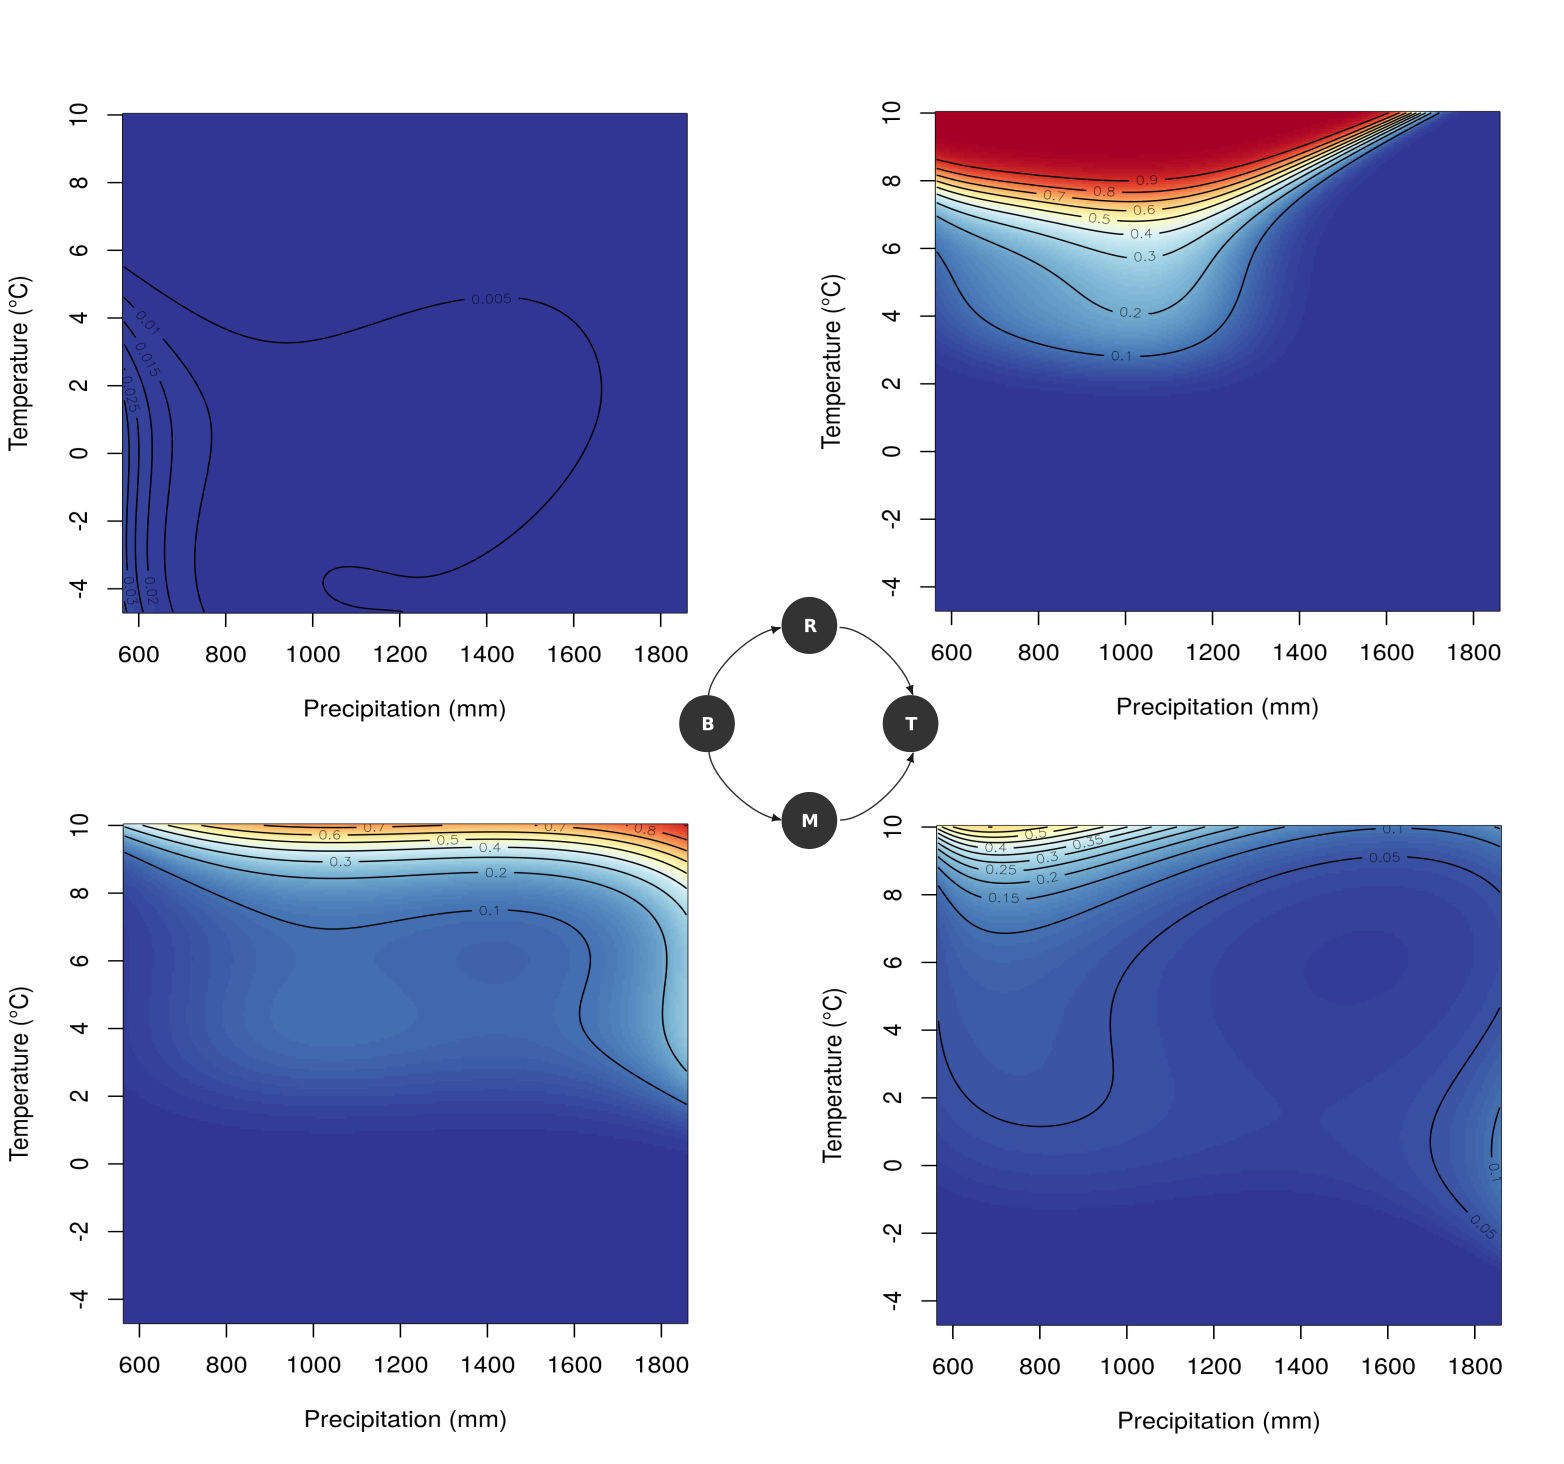
\includegraphics[width=\textwidth]{figs/trans_prob_fig1.png}
    \caption[Transition probabilities of all pathways from (B)oreal to (T)emperate]{Transition probabilities of all pathways from (B)oreal to (T)emperate. Each panel corresponds to one pathway (also represented by arrows from figure \ref{diag}). Transition probabilities were estimated by multinomial regression accounting for the temperature ($^{\circ}$C) on the y-axis and the precipitation (mm) on the x-axis.}
    \label{nnet_space}
  \end{center}
\end{figure}
\clearpage

%--------
%--------
\begin{figure}[p]
  \begin{center}
  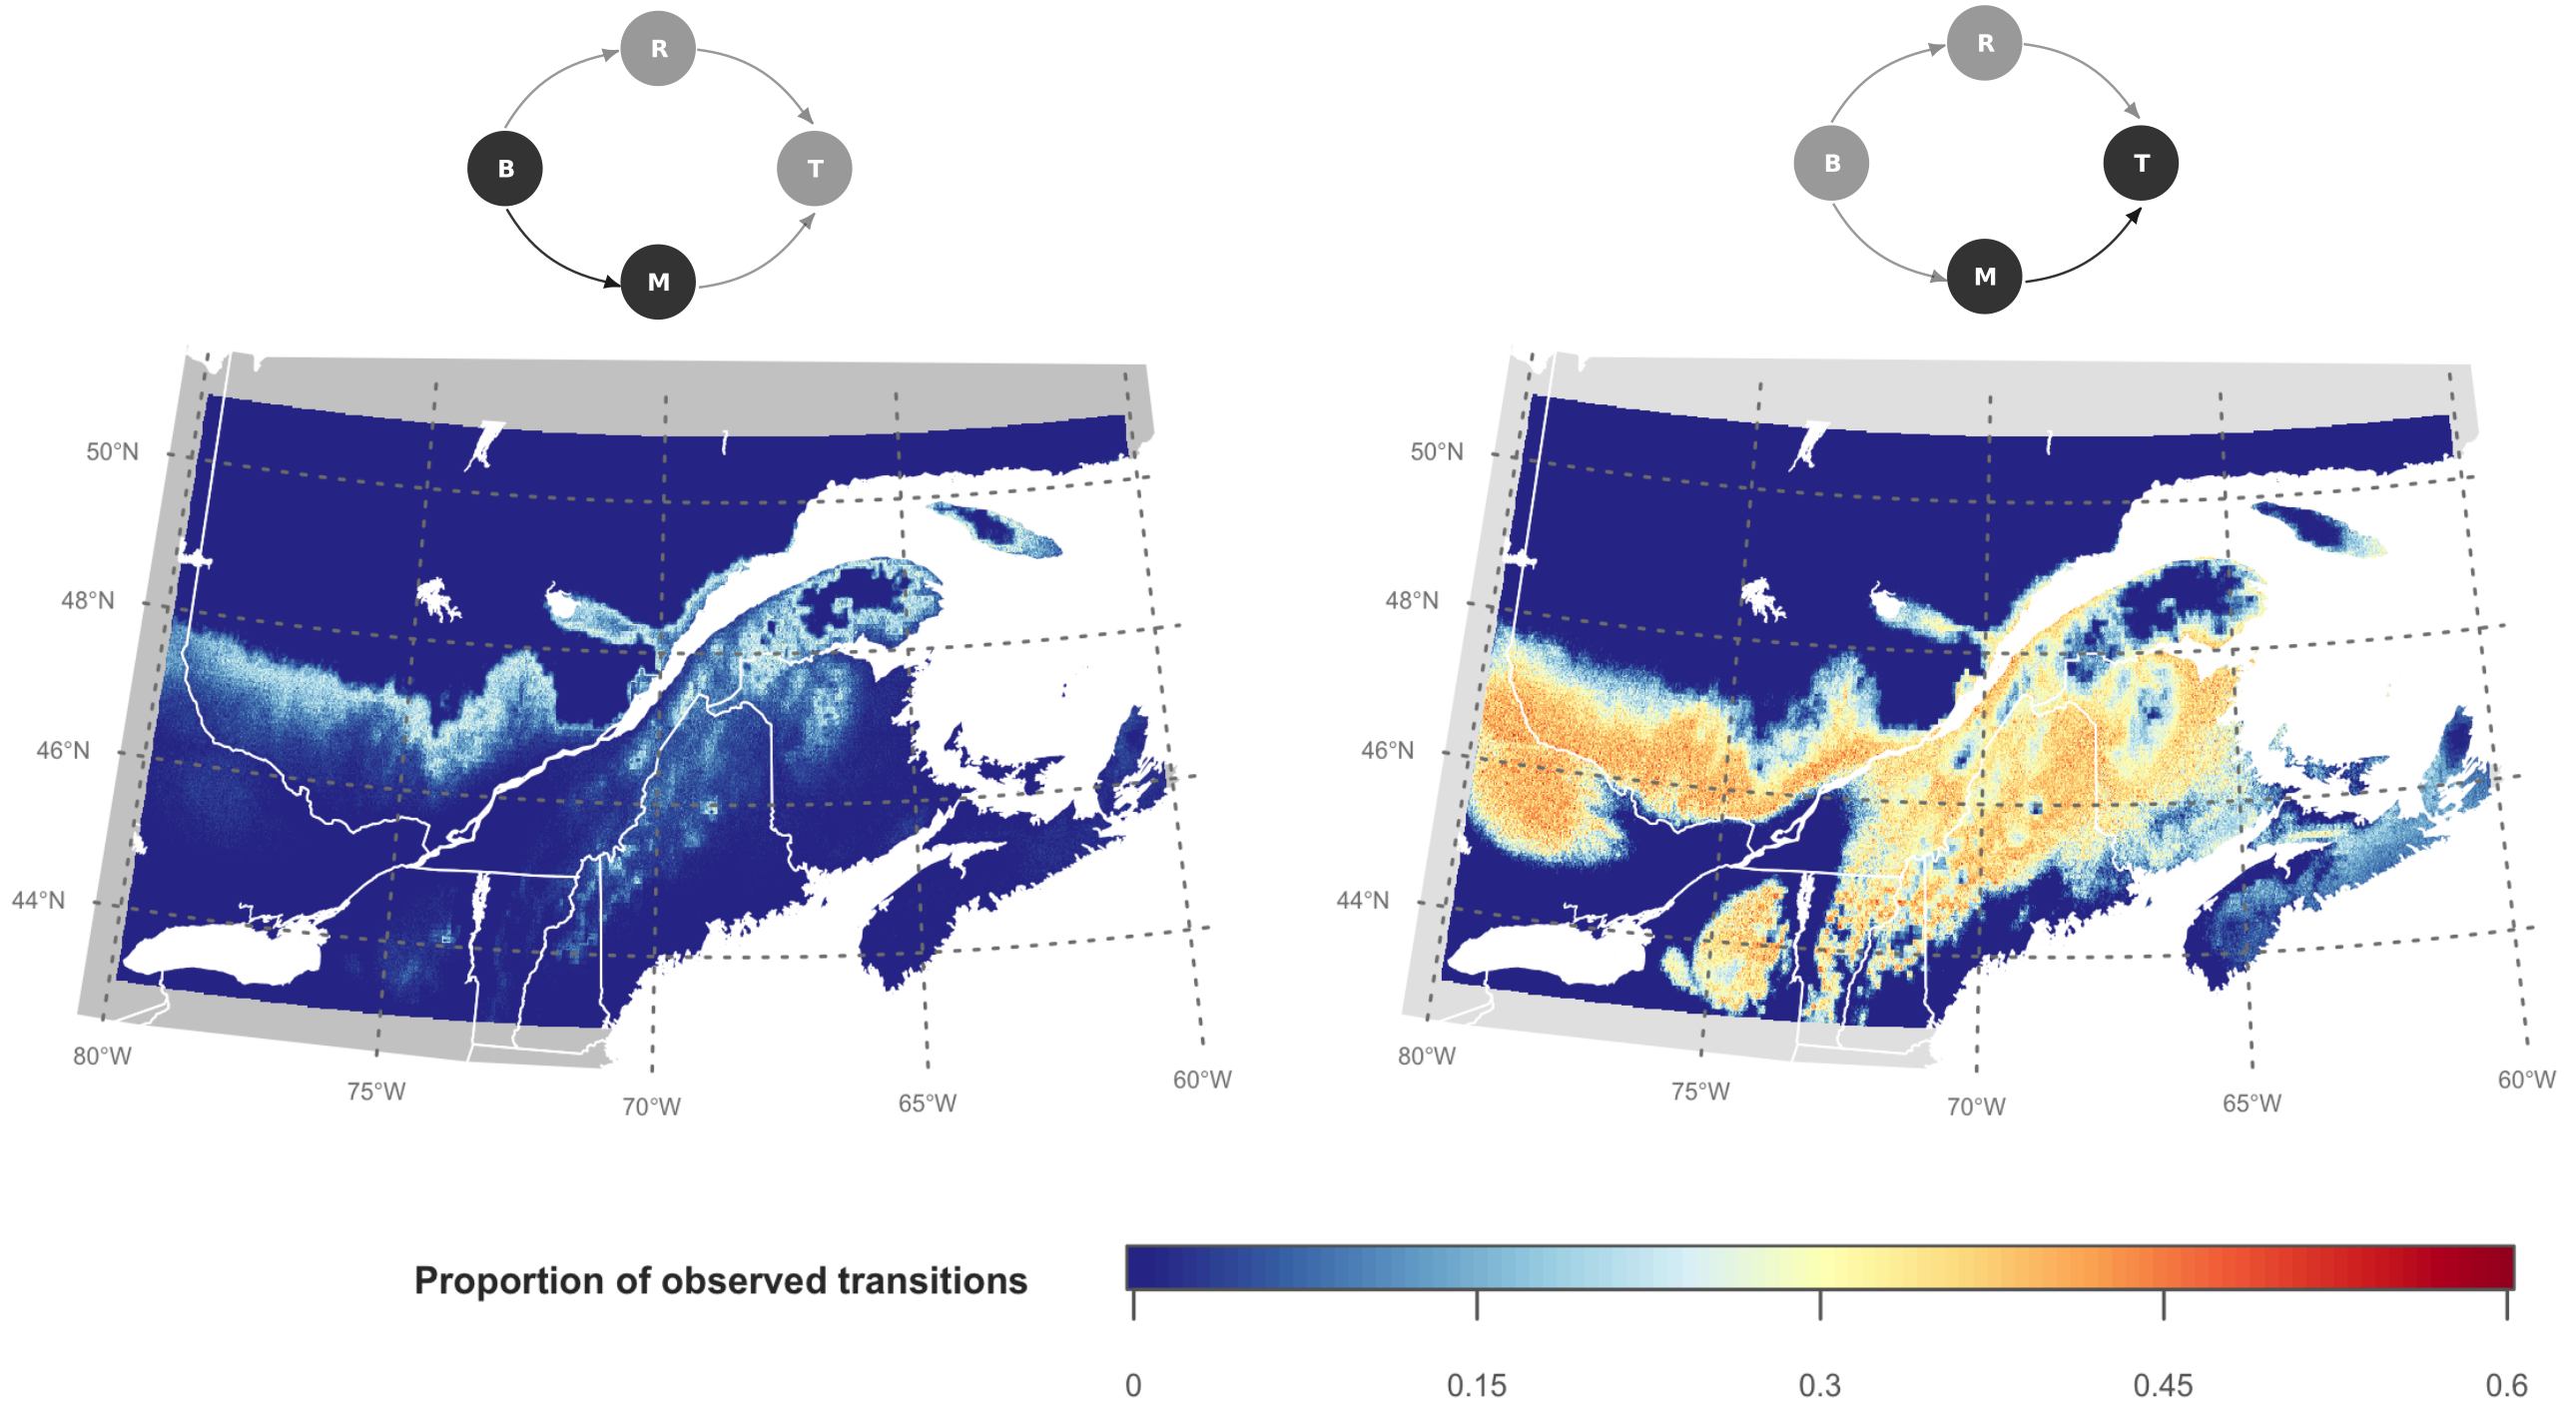
\includegraphics[width=\textwidth]{figs/turnover_states.png}
    \caption[Frequency of transitions from (B)oreal to (M)ixed and (M)ixed to (T)emperate forest  between initial (2015) and final (2095) time steps]{Frequency of transitions from (B)oreal to (M)ixed (left panel) and (M)ixed to (T)emperate forest (right panel) between initial (2015) and final (2095) time steps.
    Transitions frequencies were obtained by dividing the number of transition observed by the number of simulations. Simulations used are only based on the first model scenario accounting for dispersal limitation, biotic and demographic constraints.}
    \label{turnover}
  \end{center}
\end{figure}
\clearpage
%--------


\begin{figure}[p]
 \centering
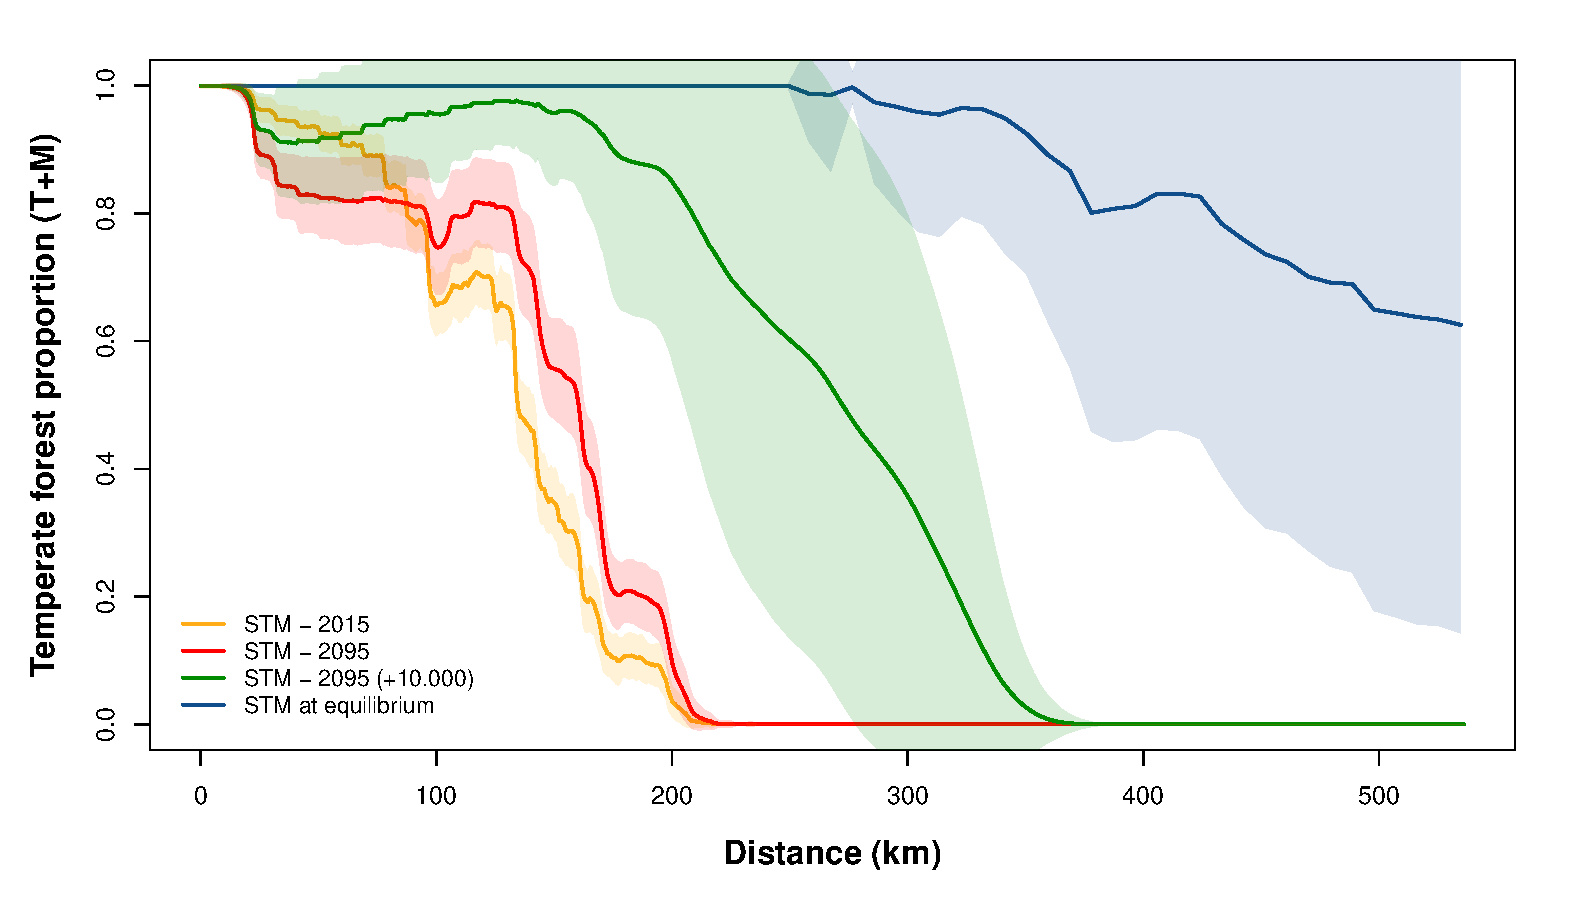
\includegraphics[width=\textwidth]{figs/propLat_wth_solved.pdf}
\caption[Mean proportion of temperate forests (with 95\% quantiles) along a 520-km latitudinal band (in km,
relative to the southernmost location of the band) showing the influence of dispersal and
demographic constraints as well as long-term dynamics]{
Mean proportion of temperate forests (with 95\% quantiles) along a 520-km latitudinal band (in km,
relative to the southernmost location of the band) showing the influence of dispersal and
demographic constraints as well as long-term dynamics. We show the results of four modelling
scenarios. The predictions of the STM for current climate (STM -- 2015; yellow) is the best estimate
of the current state of the system including dispersal and demographic constraints. When this
constrained model is projected into the future with climate change (STM -- 2095; red), we find very
little increase in the proportion of temperate forest. When the constrained model is run for 10,000
years at 2095 climate (STM -- 2095 + 10000; green), we see much greater movement, demonstrating that
dispersal and demographic constraints introduce significant lags. Finally, the model solved at
equilibrium (STM at equilibrium; blue) reveals that temperate forest will eventually expand to the
entire gradient, but that this equilibrium is considerably farther than what was reached even with
10,000 years of simulation.}
\label{mig_lat}
\end{figure}

\cleardoublepage

\section*{\uppercase{Tables}}
\vfill
\begin{table}[h]
\centering
\caption[Summary of the results of a multinomial regression estimating the relative contributions of mean annual temperature ($\text{tp}$) and total annual precipitation ($\text{pp}$) to transitions to each of the four states ($\text{X}_{t+1}$), with samples sizes $n$]{Summary of the results of a multinomial regression estimating the relative contributions of mean annual temperature ($\text{tp}$) and total annual precipitation ($\text{pp}$) to transitions to each of the four states ($\text{X}_{t+1}$), with samples sizes $n$.
We show the influence of each component of a third-order polynomial as the change in AIC ($\Delta \text{AIC}$) that results from removing the parameter from the model, where a larger value indicates a more important parameter and where $\Delta \text{AIC} > 10$ indicates strong support for a parameter \citep{Burnham:2002tk}.
To account for uneven observation intervals, we also included the time interval as a parameter in the model (and show its contribution as $\Delta \text{AIC}_{\text{time}}$).
We also show Mc-Fadden $\text{pseudo-}R^{2}$ as an indication of the goodness-of-fit of the full model.}
\label{nnet_tab}
\resizebox{\textwidth}{!}{\begin{tabular}{lccccccccccc}
\hline
\hline
  $\text{X}_{t+1}$ & $n$ & $\Delta \text{AIC}_{\text{tp}}$ & $\Delta \text{AIC}_{\text{tp}^2}$ & $\Delta \text{AIC}_{\text{tp}^3}$ & $\Delta \text{AIC}_{\text{pp}}$  &
  $\Delta \text{AIC}_{\text{pp}^2}$ &  $\Delta \text{AIC}_{\text{pp}^3}$
  &  $\Delta \text{AIC}_{\text{tp:pp}}$ &  $\Delta \text{AIC}_{\text{time}}$ & $AIC_{tot}$ & $R^{2}$\\
\hline
T &16173 & 88.32 & 0.71 & 3.85 & -2.10 & 1.10 & -2.82 & 3.08 & 98.06 & 6757.46 & 0.15\\
M & 16175 & 1.09 & 17.96 & 7.10 & 28.60 & -0.70 & 8.48 & 8.64 & 301.24 & 12034.80 & 0.04\\
R & 503 &15.43 & 48.21 & 12.69 & -5.91 & 7.54 & -0.74 & 0.06 & 18.34 & 1546.64 & 0.22\\
B & 16144 & 26.89 & 159.57 & 42.68 & -2.94 & 17.69 & 1.31 & -3.47 & 305.03 & 9013.28 & 0.11\\
\hline
\end{tabular}}
\end{table}
\vfill
\clearpage

\begin{table}[p]
\centering
\caption{Classification skill (TSS) for each state, where correct presences and absences indicate a predicted presence and absence and an observation that matched the predictions, and false presence/absence is the opposite.}
\label{validation_tab}
\begin{tabular}{ rlllll }
\hline
	& \textbf{B} & \textbf{T} & \textbf{M} & \textbf{R} & \textbf{Total} \\
  \hline
  \hline
	a. Correct presences & 1380 & 6179 & 980  & 0     & 8539 \\
	b. False presences   & 1940 & 1141 & 2175 & 285   & 5541 \\
	c. False absences    & 830  & 3062 & 1648 & 0     & 5540 \\
	d. Correct absences  & 9930 & 3698 & 9277 & 13795 & 36700 \\
	\texbf{N}            & 3320 & 7320 & 3155 & 285   & 14080 \\
  \hline
	\textbf{TSS}      & 0.46 & 0.43 & 0.18 &       & 0.48 \\
	Proportion correct (a+d/N) & 0.80 & 0.70 & 0.73 & 0.98 & 0.80 \\ \hline
\end{tabular}
\end{table}

\clearpage
%------------------------------
%-----------------------------

\section*{\uppercase{Supplementary materials}}
\setcounter{figure}{0}
\setcounter{table}{0}

\makeatletter
\renewcommand{\thefigure}{S\@arabic\c@figure}
\renewcommand{\thetable}{S\@arabic\c@figure}
\makeatother

\begin{landscape}
\hfill
\begin{figure}[h]
  \begin{align*}
    \frac{dT}{dt} &= R \cdot \alpha_T(T+M)[1-\alpha_B(B+M)] + M \cdot \theta\cdot \theta_T (1-\epsilon) - T \cdot \beta_B(B+M)(1-\epsilon) -T \cdot \epsilon \\
    \frac{dB}{dt} &= R \cdot  \alpha_B(B+M)[1-\alpha_T(T+M)] + M \cdot \theta (1- \theta_T) (1-\epsilon) - B \cdot  \beta_T(T+M)(1-\epsilon) -B \cdot \epsilon \\
    \frac{dR}{dt} &= \epsilon(M+B+T) - R \cdot \alpha_B(B+M)[1-\alpha_T(T+M)] - R \cdot \alpha_T(T+M)[1-\alpha_B(B+M)] - R \cdot \alpha_B(M + B) \alpha_T(M + T)\\
    \frac{dM}{dt} &=  B \cdot \beta_T(T+M)(1-\epsilon) +  T \cdot \beta_B(B+M)(1-\epsilon) + R \cdot \alpha_B(B+M)[1-\alpha_T(T+M)] - M \cdot \theta \cdot \theta_T (1-\epsilon) - M \cdot \theta (1- \theta_T) (1-\epsilon) - M \cdot  \epsilon\\
  \end{align*}
  \caption[Differential equations representing the boreal-temperate ecotone dynamic through the time]{Differential equations representing the boreal-temperate ecotone dynamic through the time.
  The rate of change in the proportion of patches occupied by each of the four forest states (T, B, R, and M for temperate, boreal, regenerating, and mixed forest, respectively) is a function of the local proportion of each of those states (again, T, B, R, and M) as well as the climate-specific transition parameters for each transition (Greek symbols; see main text and figure \ref{diag} for an explanation and diagrammatic representation).}
  \label{EqSys}
\end{figure}
\hfill
\end{landscape}
\clearpage

\begin{table}[p]
	\begin{center}
		\caption{Number of transitions observed between all paired observations.}
		\label{transmat}
		\begin{tabular}{c|cccc}
			 \diagbox{From}{To} &	\textbf{B} &     \textbf{M} &     \textbf{R} &     \textbf{T} \\
			\hline
			\textbf{B} & 15357 &   794 & 203 &     0 \\
			\textbf{M} &   302 & 14433 &  51 &   959 \\
			\textbf{R} &   485 &    57 & 209 &    80 \\
			\textbf{T} &     0 &   891 &  40 & 15134
		\end{tabular}
	\end{center}
\end{table}

\clearpage

\begin{figure}[p]
  \begin{center}
    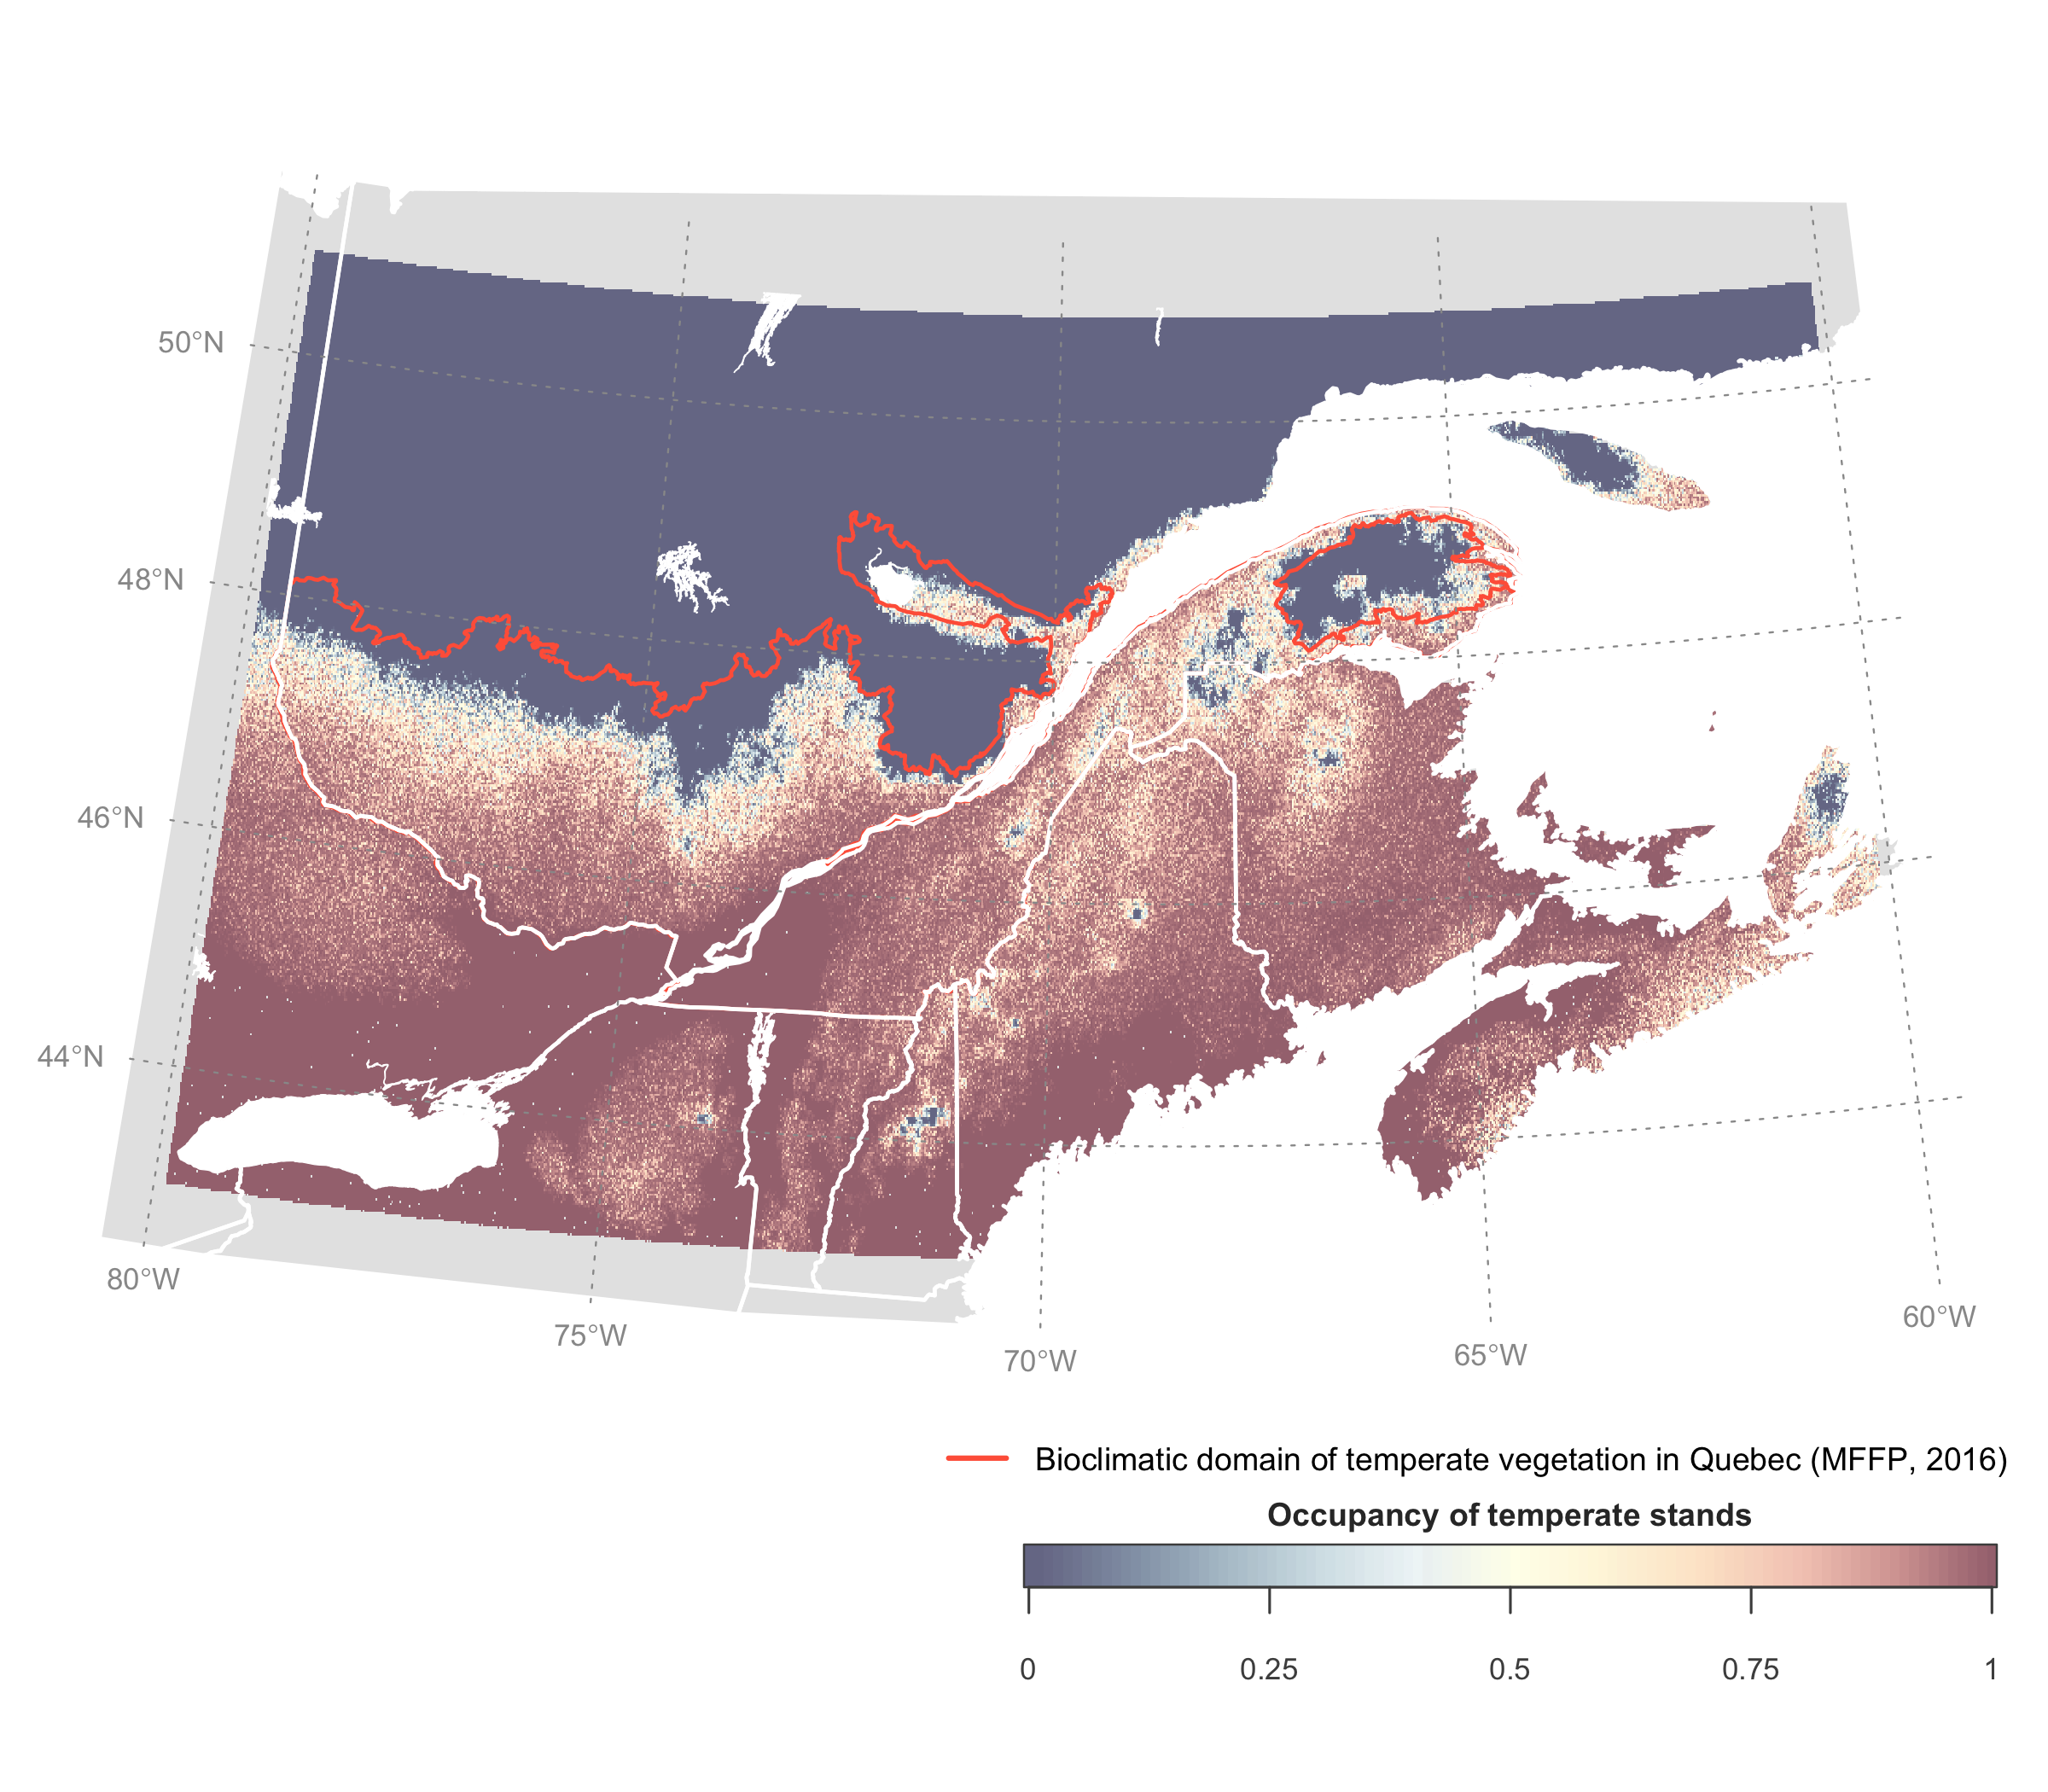
\includegraphics[width=\textwidth]{figs/pseudo_validation.png}
    \caption[The STM predictions of the present extent of temperate forest and the expert-drawn maps (provided by the forest ministry of Quebec; MFFP 2016) delineating the extent of the temperate forest bioclimatic domain]{The STM predictions of the present extent of temperate forest (colour scale) is largely concordant with expert-drawn maps (provided by the forest ministry of Quebec; MFFP 2016) delineating the extent of the temperate forest bioclimatic domain (red line), although there is some disagreement at the transition.
	Projections were made using the STM with demographic, biotic, and dispersal constraints and show the proportion of simulations where temperate or mixed forest was present.}
    \label{validation_fig}
  \end{center}
\end{figure}

\clearpage

\begin{figure}[p]
  \begin{center}
    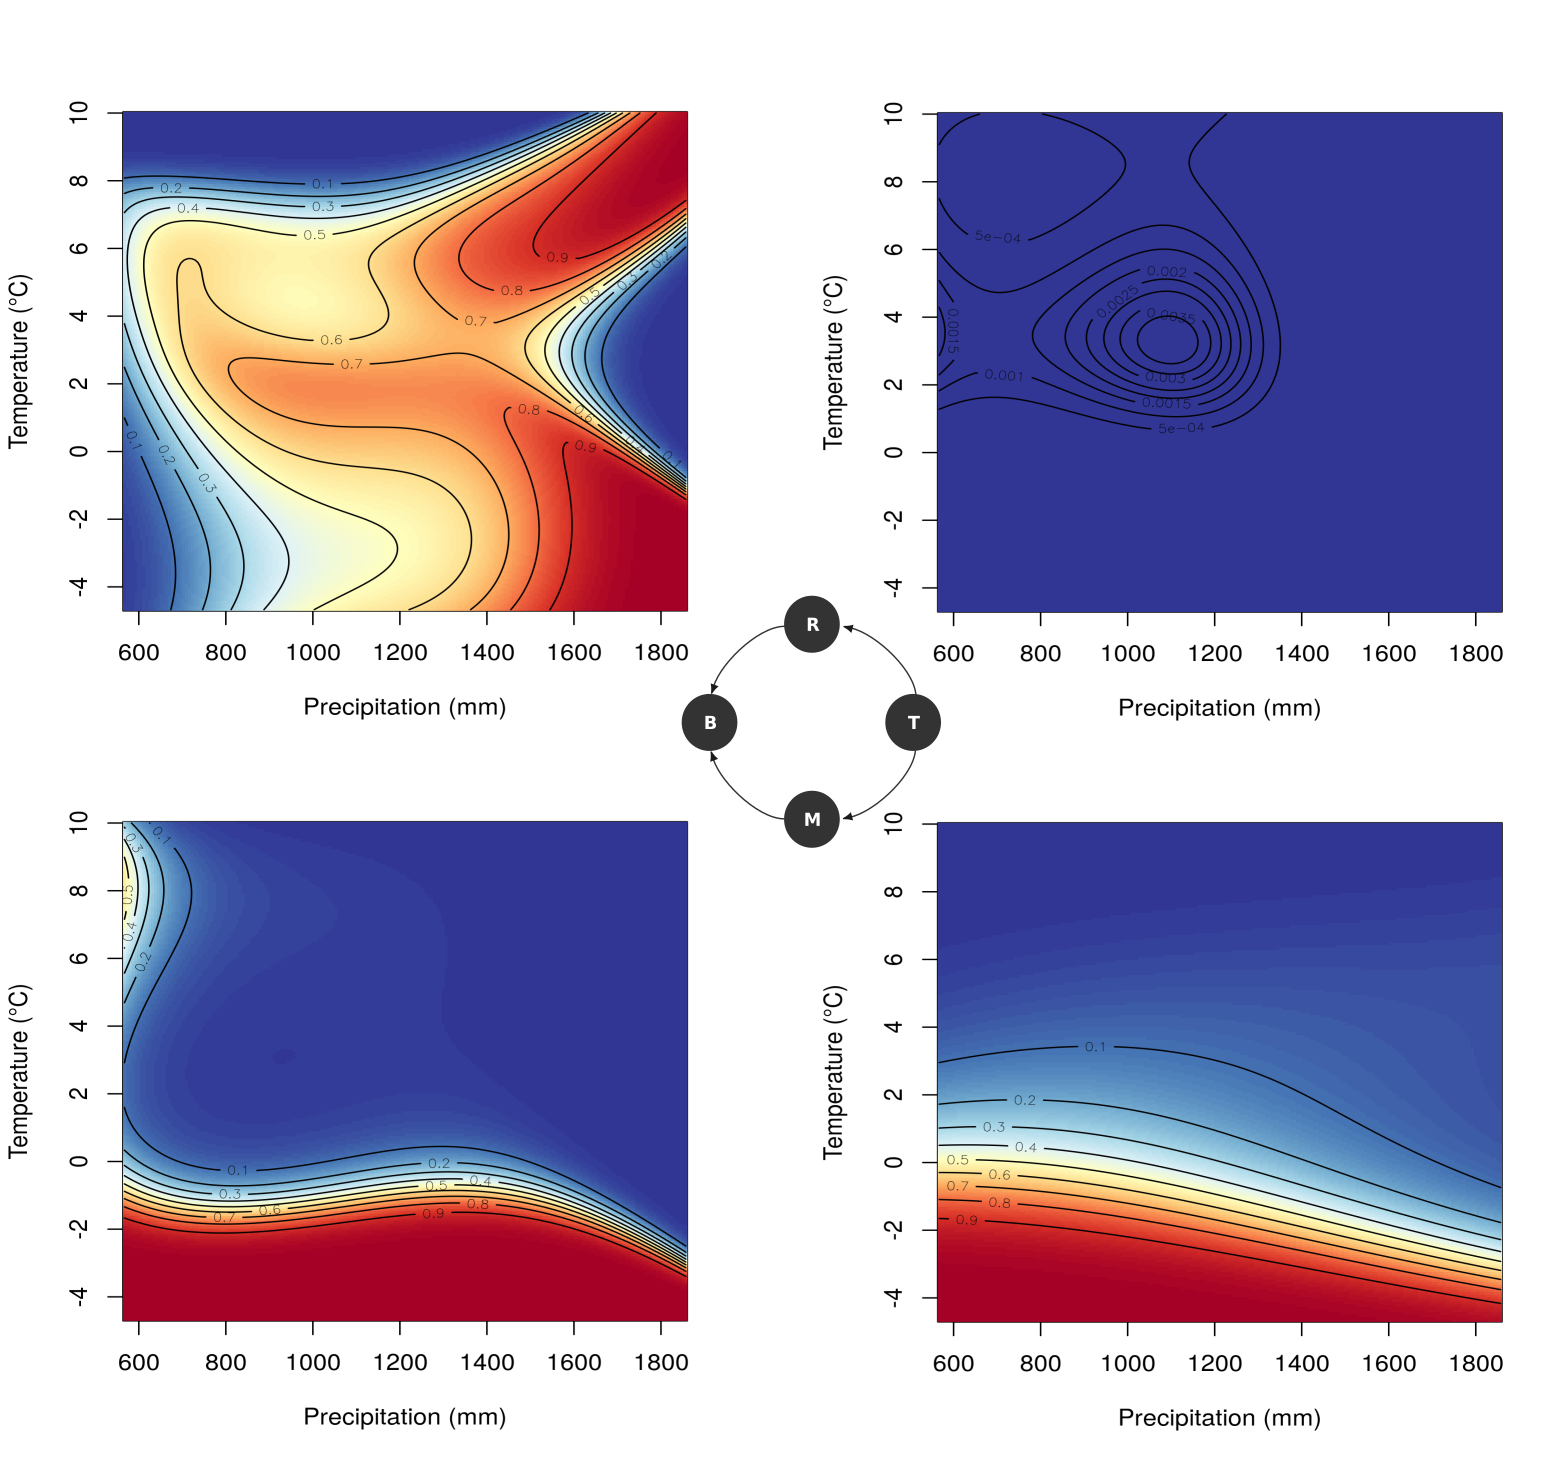
\includegraphics[width=\textwidth]{figs/trans_prob_SI.png}
    \caption[Transition probabilities of all pathways from (T)emperate to (B)oreal]{Transition probabilities of all pathways from (T)emperate to (B)oreal. Each panel corresponds to one pathway which can be attached to one arrows of the centered STM diagram (presented in figure \ref{diag}). Transition probabilities were estimated by multinomial regression accounting for the temperature ($^{\circ}$C) on the y-axis and the precipitation (mm) on the x-axis.}
    \label{nnet_space_TotB}
  \end{center}
\end{figure}

\cleardoublepage

\cleardoublepage

\conclusion
\selectlanguage{french}
[C’est dans cette section qu’est mise en évidence la portée de l’étude ainsi que les liens entre les articles ou autres textes et une ouverture sur les perspectives de recherche dans le domaine concerné. On y fait état des limites de la recherche et on y propose, le cas échéant, des pistes nouvelles pour de futures recherches ou des façons de développer de nouvelles applications. La conclusion ne doit pas présenter de nouveaux résultats ni de nouvelles interprétations. Elle doit être rédigée de manière à faire ressortir la cohérence de la démarche.]

Le modèle d'états et de transitions développé dans le cadre de cet étude a permis dévoiler que la forêt tempérée nodique ne sera pas en mesure de suivre sa niche climatique d'ici la fin du siècle. Cet incapacité est expliquable par la lente démographie des espèces tempérées et les fortes interactions biotiques avec les espèces boraéles. Ces deux composantes régissent la vitesse à laquelle les transitions des peuplements tempérée vers

Les modèles de dynamique de la végétation
(\textit{Dynamic vegetation models}, DVMs) permettent de combler certaines de ces limites par des
approches plus mécanistiques \citep{Snell2014a}. Ils intègrent par exemple la phénologie des espèces
\citep{Letters2001,Morin2008}, ou encore leurs capacités de dispersion \citep{Nobis2014,Iverson2004}
et peuvent ajouter une composante démographique \citep{Lischke2006a,Vanderwel2014}. Ces modèles
améliorent la qualité des prédictions, mais ne s'interressent pas à la contribution de chaque
mécanisme écologique (dispersion, interaction biotiques et démographie) afin de mieux comprendre
leurs effets sur la capacité d'expansion de l'aire de distribution d'une espèce ou d'une
communautée. Nous avons développés à travers cet étude une nouvelle méthologie permettant de tester

Limites du modèle:
Postulat
- Change in species assenblage
- Evolution of the niche, taille de la niche peut changer dans le temps

Contribution sur le plan écologique
- Comprendre et prédire la dynamique spatiale de l'écotone
- Importance pour les aménagistes
- Adaptation aux CC
- Aménager pour une cible en mouvement

Contribution sur le plan méthodologique
- Simplicité du modèle
- Modèle qui inclus implicitement la démographie (proba), les interaction biotiques (cells), distance de colonisation.
- Étendre la théorie des métapops à la biogéo

\cleardoublepage

% ----------------------------------------------------------------------%
% 4 - Appendices de la thèse.                                           %
% ----------------------------------------------------------------------%

\setstretch{1.5}
\selectlanguage{french}
\appendice{Titre de la première annexe}
\addtocounter{chapter}{1}
\setcounter{equation}{0}

[Cette page est facultative; l’éliminer si elle n’est pas utilisée. Une annexe est jointe lorsqu’une information pertinente (tableau, figure ou autre) risque de nuire à la compréhension du texte principal ou encore de l’alourdir inutilement. Les annexes portent un titre (même mise en page que les chapitres) et sont numérotées en chiffres romains majuscules, s’il y en a plus d’une. On y fait référence dans le texte principal par la mention « voir ». Ex. : (voir annexe I).]


\cleardoublepage

% ----------------------------------------------------------------------%
% 5 - Bibliographie.                                                    %
% ----------------------------------------------------------------------%

\begin{singlespace}
  \makeatletter
  \phantomsection\addcontentsline{toc}{chapter}{\MakeUppercase{\@references}}
  \makeatother
  \selectlanguage{english}
  \bibdata{mylib}
  \bibliographystyle{elsarticle-harv} % Ici éditer le style
  \bibliography{mylib} % Ici mettre le nom de la biblio, ici mylib.bib
\end{singlespace}

% ----------------------------------------------------------------------%
% Fin du document.                                                     %
% ----------------------------------------------------------------------%

\end{document}
